\chapter{从头学习快速生成器}\label{ch:fast-scratch}

\epigraph{
    \textit{真理总是在简单中找到，而不是在事物的多样性和混乱中找到。
}}{艾萨克·牛顿}


在\Cref{ch:distillation}中，我们看到扩散模型中的慢速迭代采样器可以通过蒸馏压缩为少步生成器。从工程角度来看，两阶段管道是实用的，因为它们将复杂的生成训练任务划分为清晰、独立的目标。第一阶段学习数据分布，第二阶段加速采样或提高质量。这种分离允许每个阶段独立优化，使整个系统更易于管理、更稳定、更可靠。

本章讨论能否从头训练一个快速生成器。
\begin{question}
    我们能否设计一个独立的生成原理，以稳定高效的方式进行训练，快速采样，并允许用户轻松指导或控制生成的内容？
\end{question}
在本章中，我们追求这个方向并讨论另一种方法：
依靠预先训练的模型训练基于扩散的几步生成器 \emph{without}。
我们的重点是 \emph{ 流映射模型 }。这里，\emph{流映射}是
ODE 的经典解映射，一个植根于微分的概念
方程和动力系统紧密相连，处于连续体和
流体力学，跟随材料颗粒的运动。
具体来说，$\bPsi_{s\to t}$ 将时间 $s$ 的状态变为
在规定的动态下于时间 $t$ 达到。流映射模型
学习直接近似该映射，从而允许长轨迹
在一个或几个网络评估中被遍历
\footnote{参见 \Cref{eq:flow-map-def} 和周围的讨论
流映射的数学和历史背景。}。






该公式提供了一种将概率质量从先验分布 $p_{\mathrm{prior}}$ 传输到数据分布 $p_{\mathrm{data}}$ 的原理方法，
同时保留每个中间时间的前向扩散过程指定的边缘分布 $p_t$。


\chapterlearning{

  \item 将瞬时速度场与其 ODE 解映射（流映射）区分开来；

  \item 了解精确 ODE 流的半群性质以及它如何激发基于一致性的学习目标；

  \item 将一致性模型、一致性轨迹模型和平均流理解为学习特殊或通用流映射的代表性方法；

  \item 将预言流映射恒等式与其实际近似值区分开来，并了解合适的参数化如何在保留对本地速度信息的访问的同时实现几步生成。

}{本章的中心对象是 ODE 流映射。各个方法应被视为用于学习同一底层对象的不同参数化和训练策略。}

\newpage
\section{序言}

\begin{figure}[th]
  \centering
  \resizebox{0.95\linewidth}{!}{
    \begin{tikzpicture}[x=2.6cm,y=1cm,line cap=butt]
      \tikzset{>={Stealth[length=12pt,width=16pt]}}
      \def\DotR{3pt}
      \def\LabelAngle{45}
      \def\DateAbove{4pt}
      \def\TextBelow{16pt}
      \newcommand{\nl}{\\}

      % Axis
      \draw[ultra thick,-Stealth] (0,0) -- (6.5,0);

      % IMPORTANT: no trailing comma on the last item
      \foreach \x/\date/\desc in {
        0.5/{2021/01}/{{\color{PersA}{KD}}\nl{\color{PersA}{Section~\ref{sec:distillation-prologue}}}},
        1.6/{2022/02}/{{\color{PersA}{PD}}\nl{\color{PersA}{Section~\ref{sec:PD}}}},
        2.7/{2023/03}/{{\color{PersA}{CM}}\nl{\color{PersA}{Section~\ref{sec:discrete-cm}}}},
        3.8/{2023/10}/{{\color{PersB}{CTM}}\nl{\color{PersB}{Section~\ref{sec:CTM}}}},
        4.9/{2024/10}/{{\color{PersA}{sCM}}\nl{\color{PersA}{Section~\ref{sec:conti-cm}}}},
        6.0/{2025/05}/{{\color{PersB}{MF}}\nl{\color{PersB}{Section~\ref{sec:MF}}}}% <-- NO COMMA HERE
      }{
        % dot
        \fill[black] (\x,0) circle[radius=\DotR];
        % date above
        \node[above=\DateAbove,align=center] at (\x,0) { \date};
        % text below (use shortstack; \nl expands to \$
        \node[below=\TextBelow,anchor=north,rotate=\LabelAngle,inner sep=1pt] at (\x,0)
          {\shortstack[c]{\strut \desc}};
      }
    \end{tikzpicture}
  }
\caption{\textbfs{基于扩散的学习流映射的方法的时间线。}\;
底层流映射是经典的ODE解映射；此处显示的日期仅指蒸馏、近似或学习该映射的现代机器学习方法。我们使用 {\color{PersA}蓝色} 针对特殊情况 {\color{PersA}$\bPsi_{s\to 0}$} 和
{\color{PersB}橙色} 用于一般映射
{\color{PersB}$\bPsi_{s\to t}$}.
\figcredit{由作者创建。}}
  \label{fig:timeline}
\end{figure}




\paragraph{流映射模型的动机。}
在 \Cref{ch:distillation} 我们展示了 oracle flow-map 中不可访问的回归目标如何丢失
$\mathcal{L}_{\mathrm{oracle}}(\btheta)$ （参见 \Cref{eq:general-cm-loss:rep}) 可以通过从预先训练的扩散模型中提取知识来估计，以获得少步生成器。这条路线有效且实用：可以设计两级管道以实现稳健性，并且通常在数据和计算效率方面保持竞争力。在本章中，我们将重点转向深度生成模型研究中一个更广泛的挑战：
\emph{我们能否建立一个独立的生成原理，实现稳定、可扩展、高效的训练、快速采样和生成，并且可以根据用户意图轻松引导，而不依赖于预先训练的模型？}
设计这种独立的原则是生成建模的核心。扩散模型提供了一个有用的设计原则：从连续时间前向过程开始，逐渐将数据转换为简单的先验（噪声）作为参考，并将建模任务框架为学习逆时传输，恢复该过程以匹配所需的边缘分布。与一次性生成图相比，这种依赖于时间的公式还可以更轻松地在中间步骤引导生成过程。专门针对扩散驱动的方法，这引出了一个问题：
\begin{question}
我们可以学习流映射吗 $\bPsi_{s\to t}(\cdot)$ 带网络
$\rmG_\btheta(\cdot,s,t)$ (a \emph{流映射模型}）无需访问预训练模型，同时保持高保真生成？
\end{question}
\begin{figure}[th!]
    \centering
    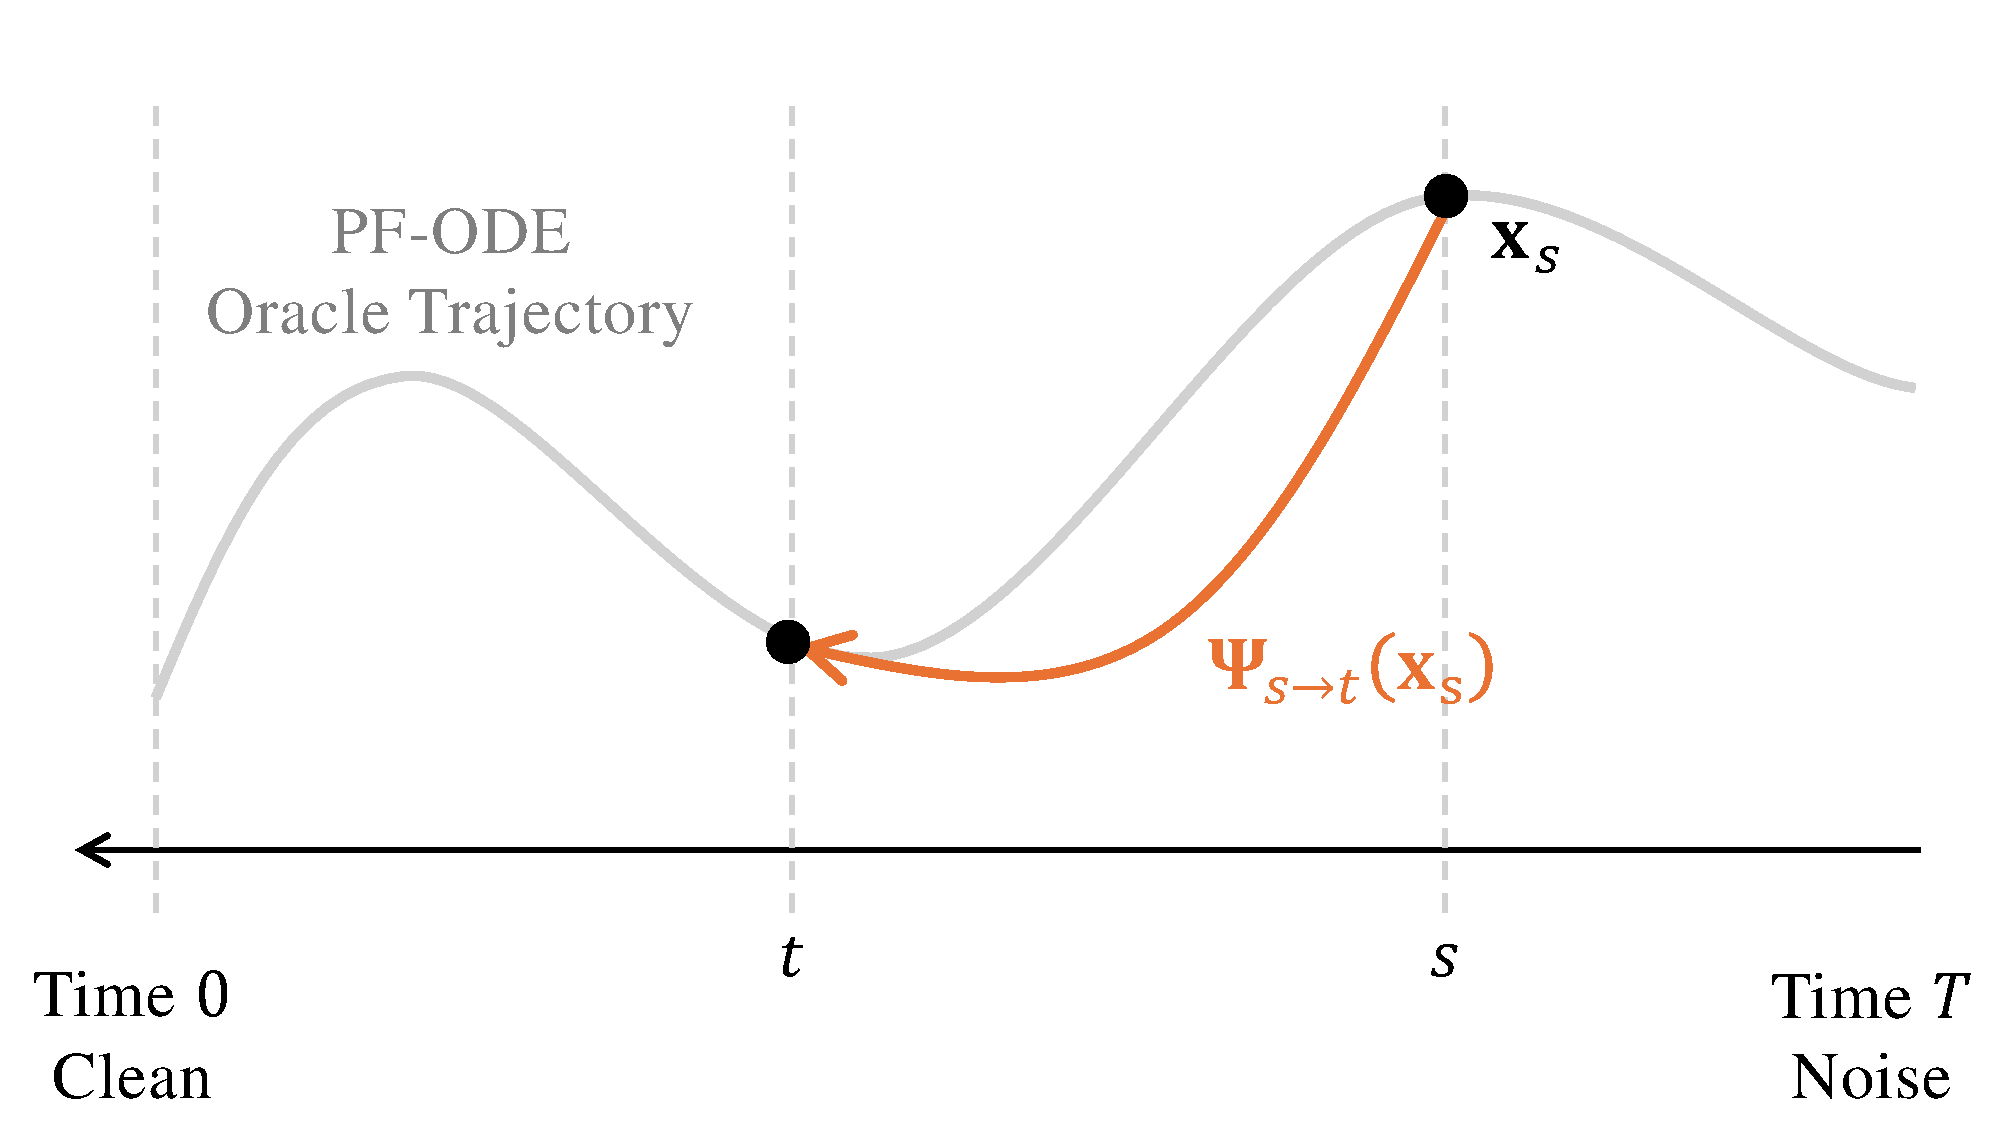
\includegraphics[width=0.9\linewidth]{Images/PartD/flow-map.pdf}
    \caption{\textbfs{流映射的插图。} 从任何状态开始 $\rvx_s$ 当时 $s$，流映射 $\bPsi_{s \to t}$ 将其传送到同一个PF-ODE预言机轨迹上的对应点 $t$. \figcredit{由作者创建。}}
    \label{fig:flow-map-illustration}
\end{figure}


本章开发了实现这一目标的方法，这些方法围绕一个单一目标进行组织，该目标也是蒸馏的基础，并提供了流映射公式的统一视图~\citep{boffi2024flow,hu2025cmt}:
\begin{mdframed}
\begin{equation}\tag{\ref*{eq:general-cm-loss}}\label{eq:general-cm-loss:rep}
  \mathcal{L}_{\mathrm{oracle}}(\btheta)
  := \mathbb{E}_{s,t}\,\mathbb{E}_{\rvx_s \sim p_s}\Big[
     w(s,t)  d\big(\rmG_\btheta(\rvx_s,s,t),  \bPsi_{s\to t}(\rvx_s)\big)
  \Big].
\end{equation}
\end{mdframed}

\addtocounter{equation}{-1}
这里 $s,t$ 是从某个时间分布（例如均匀分布）中采样的，
$w(s,t) \ge 0$ 为时间对 $(s,t)$ 和 $d(\cdot,\cdot)$ 分配权重
是差异度量，例如 $\ell_2$ 范数的平方。预言机流映射
$\bPsi_{s\to t}$ 表示采用状态的理想变换
$\rvx_s$ 在时间 $s$ 并将其直接传输到时间 $t$：
\[
\bPsi_{s\to t}(\rvx_s) = \rvx_s + \int_s^t \rvv^*(\rvx_u,u)\,\mathrm{d}u,
\]
其中预言漂移给出为
\[
\rvv^*(\rvx_u,u) = \E \left[\alpha_u'\rvx_0+ \sigma_u'\beps | \rvx_u\right],
\]
而等效的参数化也是可能的（参见 \Cref{ch:all-equivalent}），常见的选择包括 $\rvx$ 预测和 $\rvv$ 预测形式。 

在预言机损失最优时，学习模型恢复真实的流映射
确切地说：
\[
\rmG^*(\rvx_s, s, t) = \bPsi_{s\to t}(\rvx_s), \quad \text{for all }\, s,t, \text{ and }\, \rvx_s \sim p_s.
\]


由于流映射 $\bPsi_{s\to t}$ 无法以封闭形式表示，因此必须对其进行近似。 
\Cref{ch:distillation} 中讨论的一种选择是依赖预先训练的扩散模型。 
或者，正如我们将在本章中看到的，可以引入新的、更容易处理的替代物。 
为了清楚起见，现有的方法可以根据训练过程是否在循环期间询问教师来大致分类： 
\emph{distillation}，明确调用教师模型，以及 
\emph{从头开始训练}，通过构建独立的代理来避免教师调用。



在此原则的基础上
目标，我们现在转向学习流映射模型的系统方法，
旨在开发实用的方法，同时也能生产
更准确地反映真实数据分布的世代
计算效率高。我们首先对这个范例进行高级介绍。
\paragraph{特殊流映射：一致性函数.}
\emph{一致性模型}~\citep{song2023consistency}代表了最早的流映射学习开创性方法之一。 
他们学习了一个几步降噪器 $\rvf_\btheta(\cdot,s)$，该降噪器将流映射的特殊情况近似到原点：
\[
\bPsi_{s\to 0}(\cdot), \qquad s \in (0,T].
\]
关键思想是每个状态 $\rvx_s$ 都映射到时间 $0$ 端点
通过它的 PF-ODE 轨迹为 $\bPsi_{s\to 0}(\rvx_s)$。形式上，CM家族的预言机训练目标~\citep{song2023consistency,songimproved,geng2024consistency,lu2024simplifying}是
\begin{align}\label{eq:oracle-cm}
    \mathcal{L}_{\methodl{oracle}{CM}}(\btheta) 
    := \E_{s} \E_{\rvx_s\sim p_s} \left[ w(s)  d \left(\rvf_\btheta(\rvx_s,s), \bPsi_{s\to 0}(\rvx_s)\right)\right].
\end{align}




但实际上，oracle $\bPsi_{s\to 0}(\rvx_s)$ 不可用。因此，它被替换为 \emph{stop-gradient} 目标，表示为 $\rvf_{\btheta^-}$，取自同一轨迹上稍早的步骤 $\bPsi_{s\to s-\Delta s}(\rvx_s)$：
\[
\bPsi_{s\to 0}(\rvx_s) \approx \rvf_{\btheta^-} \left(\bPsi_{s\to s-\Delta s}(\rvx_s),\,s-\Delta s\right), \quad \Delta s > 0,
\]
其中 $\bPsi_{s\to s-\Delta s}(\rvx_s)$ 本身也必须近似。两个
实用的策略有：（i）\emph{distillation}，它依赖于
预训练的扩散模型，以及（ii）\emph{从头开始训练}，它使用
没有教师模型指导的一点估计。

\paragraph{一般流映射。} 两种代表性方法是 \emph{一致性轨迹模型} （CTM）和 \emph{平均流} （MF）。
\subparagraph{一致性轨迹模型。} \emph{一致性轨迹模型} （CTM）\\~\citep{kim2023consistency} 是学习通用流映射的第一个作品 $\bPsi_{s\to t}$ 任意开始和结束时间，可以看作是统一目标下的具体实例 \Cref{eq:general-cm-loss:rep}。 CTM 采用欧拉启发的参数化，将预言流映射表示为
\begin{align*}
\bPsi_{s\to t}(\rvx_s)
:= \rvx_s + \int_s^t \rvv^*(\rvx_u,u)\diff u 
= \frac{t}{s} \rvx_s
+ \frac{s-t}{s}
\underbrace{\Big[\rvx_s + \frac{s}{s-t} \int_s^t \rvv^*(\rvx_u,u) \diff u\Big]}_{\approx~\rvg_{\btheta}},
\end{align*}
激发神经参数化
\[
\rmG_{\btheta}(\rvx_s,s,t)
:= \frac{t}{s}\,\rvx_s + \frac{s-t}{s}\,\rvg_\btheta(\rvx_s,s,t),
\]
其中 $\rvg_\btheta$ 是一个经过训练的神经网络 $\bPsi_{s\to t}(\rvx_s)\approx \rmG_{\btheta}(\rvx_s,s,t)$。自从神谕 $\bPsi_{s\to t}(\rvx_s)$ 无法访问，CTM针对a进行训练 \emph{停止梯度} 在中间时间评估的目标 $u$:
\[
\bPsi_{s\to t}(\rvx_s)
 \approx 
\rmG_{\btheta^-} \big(\bPsi_{s\to u}(\rvx_s),\,u,\,t\big),
\qquad u\in[t,s],
\]
其中中间状态 $\bPsi_{s\to u}(\rvx_s)$ 通过以下两种方式之一进行近似：(i) \emph{蒸馏}，它使用应用于预先训练的扩散教师的几步求解器，或 (ii) \emph{从头开始训练}，直接通过 $\rmG_\btheta$
参数化。


\subparagraph{平均流。}
平均流 (MF)~\citep{geng2025mean} 通过建模建立在流匹配的基础上 \emph{平均漂移} 在一段时间内 $[t,s]$ （与 $t\le s$):
\[
\rvh_{\btheta}(\rvx_s,s,t)
 \approx 
\rvh^*(\rvx_s,s,t)
:= \frac{1}{\,t-s\,}\int_s^t \rvv^*(\rvx_u,u)\,\diff u,
\]
也与 \Cref{eq:general-cm-loss:rep}。区分恒等式
\[
(t-s)\,\rvh^*(\rvx_s,s,t)  =  \int_s^t \rvv^*(\rvx_u,u)\,\diff u
\]
相对于 $s$ 产生激发 MF 目标的自引用关系
\[
\mathcal{L}_{\mathrm{MF}}(\btheta)
:= \E_s\,\E_{\rvx_s\sim p_s} \Big[w(s)\,\big\|
\rvh_{\btheta}(\rvx_s,s,t)-\rvh_{\btheta^-}^{\mathrm{tgt}}(\rvx_s,s,t)
\big\|_2^2\Big],
\]
带停止梯度目标
\[
\rvh_{\btheta^-}^{\mathrm{tgt}}(\rvx_s,s,t)
:= \rvv^*(\rvx_s,s)  -  (s-t) \left((\partial_\rvx \rvh_{\btheta^-})\,\rvv^*(\rvx_s,s) + \partial_s \rvh_{\btheta^-}\right).
\]
在实践中，预言机速度 $\rvv^*(\rvx_s,s)$ 也必须近似。两种常见的策略是：（i） \emph{蒸馏}，利用经过流匹配训练的预训练扩散模型，或 (ii) \emph{从头开始训练}，使用单点条件速度
$\alpha'_s\,\rvx_0+\sigma'_s\,\beps$ 源自前向扰动过程
$\rvx_s = \alpha_s \rvx_0+\sigma_s \beps$.



\subparagraph{CTM 和 MF 之间的关系。}
CTM 和 MF 近似相同的路径积分，但参数化它的不同代理：
\begin{align*}
\bPsi_{s\to t}(\rvx_s)
&:= \rvx_s  +  \int_s^t \rvv^*(\rvx_u,u)\,\diff u
\\[2pt]
&= \frac{t}{s}\,\rvx_s
 +  \frac{s-t}{s}\,
\underbrace{\Big[\rvx_s + \frac{s}{\,s-t\,} \int_s^t \rvv^*(\rvx_u,u)\,\diff u\Big]}_{\approx~\rvg_{\btheta} }
\\[4pt]
&= \rvx_s  +  (t-s)\,
\underbrace{\Big[\frac{1}{\,t-s\,} \int_s^t \rvv^*(\rvx_u,u)\,\diff u\Big]}_{\approx~\rvh_{\btheta} }.
\end{align*}
换句话说，CTM 学习了 \emph{斜坡位移} 通过 $\rvg_\btheta$，而 MF 学习 \emph{平均漂移} $\rvh_\btheta$;两者都是近似定义相同积分的一致方法 $\bPsi_{s\to t}$.


\paragraph{接下来会发生什么？}
我们从CM家族开始，重点关注具体的流映射
$\bPsi_{s\to 0}$。这部分涵盖了其离散时间原点
\Cref{sec:discrete-cm} 及其连续时间延长
\Cref{sec:conti-cm}。然后我们继续讨论总体流映射，并详细讨论两个关键代表：CTM 和 MF。它们的参数化、训练策略和实际近似值在 \Cref{sec:CTM} 和 \Cref{sec:MF}分别是。

我们注意到 \emph{阐明扩散模型} （EDM）引入于
\Cref{sec:edm} 为设计网络参数化提供系统指南 $\rvx$-预测模型并表现出强大的实证性能。尽管本部分可以被认为是可选的，但 EDM 公式可以作为 CM 样式模型的宝贵基础。为了后面的说明清楚起见，我们并不严格遵循这些方法出现的时间顺序。相反，我们通过概念关系来组织讨论。尽管如此，为了承认原创性并尊重时间顺序，我们提供了历史时间表 \Cref{fig:timeline}.







\clearpage
\newpage


\section{特殊流映射：离散时间的一致性模型}\label{sec:discrete-cm}

\paragraph{流映射的重要原理：半群性质。}
\begin{figure}[th!]
    \centering
    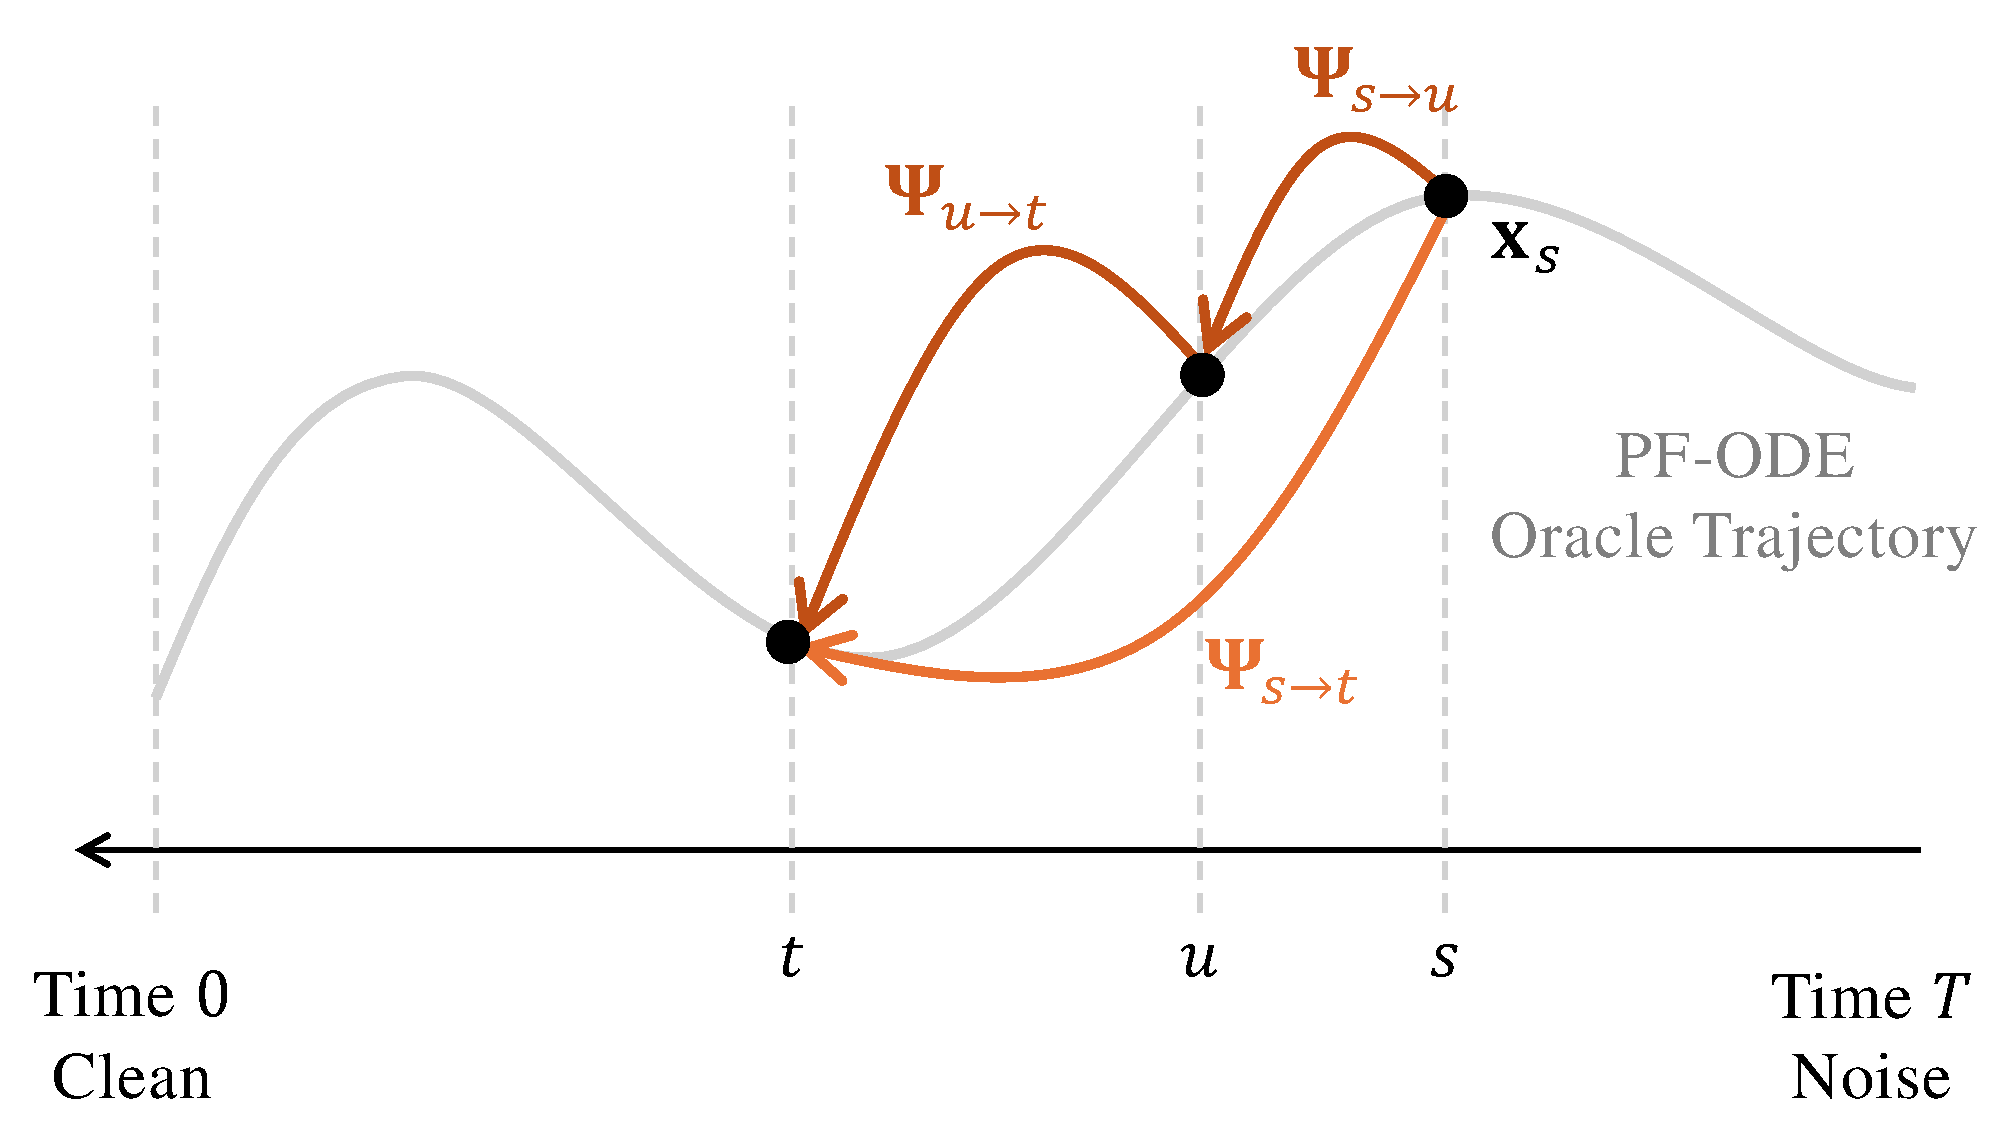
\includegraphics[width=0.9\linewidth]{Images/PartD/semigroup.pdf}
    \caption{\textbfs{流映射半群属性的图示。} 
该属性表明从 $s$ 至 $u$ 然后从 $u$ 至 $t$ 
相当于直接从 $s$ 至 $t$.
\figcredit{由作者创建。}}
    \label{fig:semigroup}
\end{figure}


一致性模型（在 \Cref{sec:discrete-cm,sec:conti-cm}) 及其概括，一致性轨迹模型 (\Cref{sec:CTM})，通过利用流映射的关键数学结构来定义回归目标。这个结构是基础 \emph{半群性质}:
\begin{mdframed}
   \begin{align}\label{eq:semi-group}
       \bPsi_{u\to t}\circ \bPsi_{s\to u}=\bPsi_{s\to t},
       \,\,\,
       \bPsi_{s\to s}=\rmI, \quad \text{for all }\, s, u, t \in [0,T].
   \end{align} 
\end{mdframed}
直观上，这意味着如果我们首先从 $s$ 至 $u$ （通过 $\bPsi_{s\rightarrow u}$) 然后从 $u$ 至 $t$ （通过 $\bPsi_{u\rightarrow t}$)，我们最终处于完全相同的点，就好像我们直接从 $s$ 至 $t$。这无非是ODE求解的基本原理\footnote{半群性质源自 ODE 初值问题的唯一性定理（请参阅 \Cref{app:de}).}: 一旦指定了流的起点，其未来的演变就完全确定，并且它遵循单一的明确定义的路径。无论我们沿着这条路径迈出一大步，还是将其分成更小的间隔，我们仍然沿着相同的轨迹移动并到达相同的最终状态。为了进一步加深对半群性质的直觉，请考虑解轨迹 $\{\rvx(s)\}_{s \in [0,T]}$ PF-ODE 的
\begin{align*}
    \frac{\diff \rvx(\tau)}{\diff \tau} = \rvv^*(\rvx(\tau), \tau),
\end{align*}
具有固定的初始条件 $\rvx(T)$ 当时 $T$，及时向后解决。如果我们将终端时间固定在 $t=0$，对应的流映射可以更简单地写为
\[
\rvf^*(\cdot, s) := \bPsi_{s\to 0}(\cdot),
\]
简称为 \emph{一致性函数}。通过构造，该函数直接从半群恒等式继承了几个基本属性 \Cref{eq:semi-group} 与 $t=0$:\begin{enumerate}
    \item[(i)] \textbfs{全局一致性：} 轨迹上的每个点都映射到相同的干净端点，
    \[
       \rvf^*(\rvx(s), s) = \rvx(0), \quad \text{for all }\, s \in [0,T].
    \]
    这是因为 
\begin{align*}
\rvf^*(\rvx(s),s)
&= \bPsi_{s\to 0}\big(\bPsi_{0\to s}(\rvx(0))\big)
= \big(\bPsi_{s\to 0}\circ \bPsi_{0\to s}\big)(\rvx(0))
\\&= \bPsi_{0\to 0}(\rvx(0))
= \rvx(0).
\end{align*}
    \item[(ii)] \textbfs{ 自洽：} 沿同一轨迹的任意两点必须给出相同的输出，
    \begin{align}\label{eq:cm-self-consistency}
       \rvf^*(\rvx(s), s) = \rvf^*(\rvx(u), u), \quad \text{for all }\, s, u \in [0,T].
    \end{align}
    这是半群恒等式的直接重新解释：$\Psi_{s\rightarrow 0}\circ\Psi_{0\rightarrow s}=\Psi_{u\rightarrow 0}\circ\Psi_{0\rightarrow u}$。
    \item[(iii)] \textbfs{局部一致性：}当沿着轨迹评估时，一致性函数相对于$s$是不变的，
    \begin{align}\label{eq:cm-diff}
        \frac{\diff}{\diff s}\,\rvf^*(\rvx(s),s) = 0,
        \qquad \rvf^*(\rvx(0),0) = \rvx(0).
    \end{align}
这是根据全局一致性得出的，其中指出 $\rvf^*(\rvx(s), s)$ 确实
沿轨迹与$s$不发生变化。
\end{enumerate}
这三个属性都是等价的。每个都表明沿着任何解决方案轨迹 $s\mapsto \rvx(s)$，
流向原点/一致性图 $\rvf^*(\rvx(s),s)=\bPsi_{s\to 0}(\rvx(s))$
产生相同的终点 $\rvx(0)$，与起始时间无关。


\paragraph{一致性模型目标.}
CM 旨在训练神经网络 
$\rvf_{\bm{\theta}} \colon \mathbb{R}^D \times [0,T] \to \mathbb{R}^D$ 
近似特殊流映射 $\bPsi_{s\to 0}$，即一致性函数 \footnote{ ODE 一致性函数的概念推广为函数
$\rvf(\rvx,t)$ 对于 SDE，使得 $\rvf(\rvx_t,t)$ 是一个（本地）鞅
尊重 SDE 的自然过滤，即
\[
\E[\rvf(\rvx_t,t)|\rvx_s]=\rvf(\rvx_s,s),\quad\text{for all }\quad t\ge s.
\]
这种概括是在 \citep{daras2023consistent,lai2023fp} 中提出/观察到的，
理论联系总结在\citep{lai2023equivalence}.}中。 
关键思想是沿着 PF-ODE 轨迹强制一致性：状态说谎
同一 ODE 轨迹上应映射到同一时间 -$0$ 端点
（更准确地说，这对应于特殊情况 $t=0$ 和
$u=s-\Delta s$ 中的 \Cref{eq:semi-group}）。

然而，有多种方法可以实现这一目标。 
选择取决于是否有预训练的扩散模型，以及训练是在离散时间还是连续时间状态下进行。 
我们首先在 \Cref{tb:consistency-methods} 中总结这些变体，并在 \Cref{fig:cd-ct-loss-distill} 中说明它们的目标。 
随后的部分 (\Cref{sec:discrete-cm,sec:conti-cm}) 将逐步详细介绍每种方法的细节。

\begin{table}[th]
  \caption{一致性模型的训练目标}
  \small
  \centering
  \resizebox{0.76\textwidth}{!}{
  \begin{tabular}{ccc}
     \toprule
     & \textbfs{蒸馏} & \textbfs{从头开始} \\
     \midrule
     \textbfs{离散时间} & \Cref{eq:cd-discrete-approx-N} & \Cref{eq:ct-discrete-approx-N} \\
     \textbfs{连续时间} & \Cref{eq:cd-continuous-time} & \Cref{eq:ct-continuous-time} \\
     \bottomrule
  \end{tabular}
  }
  \label{tb:consistency-methods}
\end{table} 




\subsection{用于学习一致性函数的离散时间近似}\label{subsec:approx-cm}

原则上，可以通过最小化预言机损失来学习一致性函数 \Cref{eq:oracle-cm}:
\[
    \mathcal{L}_{\methodl{oracle}{CM}}(\btheta) 
    := \E_{s} \E_{\rvx_s\sim p_s} \left[ w(s)  d \left(\rvf_\btheta(\rvx_s,s), \bPsi_{s\to 0}(\rvx_s)\right)\right].
\]
该目标强制每个噪声样本 $\rvx_s$ 映射回其干净端点 $\bPsi_{s\to 0}(\rvx_s)$。挑战在于预言图 $\bPsi_{s\to 0}(\rvx_s)$ 实际中不可用。为了克服这个问题， \citet{song2023consistency} 利用 \emph{半群性质}：任何噪声状态及其沿着相同 PF-ODE 轨迹的连续步骤必须映射到相同的干净端点。具体来说，oracle 目标被替换为 \emph{停止梯度} 从轨迹上稍早的点获取的目标：
\begin{align*}
    \bPsi_{s\to 0}(\rvx_s) 
    &= \bPsi_{s-\Delta s \to 0} \left(\bPsi_{s\to s-\Delta s}(\rvx_s)\right) \\
    &\approx \rvf_{\btheta^-} \left(\bPsi_{s\to s-\Delta s}(\rvx_s),\,s-\Delta s\right), 
    \qquad \Delta s > 0,
\end{align*}
其中 $\bm{\theta}^-$ 是停止梯度算子下的参数。另一个困难是中间状态 $\bPsi_{s\to s-\Delta s}(\rvx_s)$ 也没有闭形式，其本身必须是近似的。提出了两种实用的制度：

\paragraph{具有预先训练的扩散模型（一致性蒸馏）。}
假设我们可以访问预先训练的扩散模型。一致性蒸馏（CD）利用教师模型来近似中间状态 $\bPsi_{s\to s-\Delta s}(\rvx_s)$ 通过仅模拟单个向后 ODE 步骤：
\[
 \bPsi_{s\to s-\Delta s}(\rvx_s)  \approx  \mathtt{Solver}_{s \to s-\Delta s}(\rvx_s).
\]

更具体地说，预训练的扩散模型提供了分数函数的估计 
$\rvs_{\bm{\phi}^\times}(\rvx_s, s) \approx \nabla_{\rvx_s}\log p_s(\rvx_s)$。使用此功能，可以从以下位置执行一步 DDIM 更新： $\rvx_s$ 获得状态的近似值 $s' = s-\Delta s$:
\begin{align*}
    \bPsi_{s\to s-\Delta s}(\rvx_s) 
    &\approx \frac{\alpha_{s'}}{\alpha_s}\,\rvx_s 
    + \sigma_s^2 \left( \frac{\alpha_{s'}}{\alpha_s} - \frac{\sigma_{s'}}{\sigma_s} \right)\nabla_{\rvx_s}\log p_s(\rvx_s) \\
    &\approx \frac{\alpha_{s'}}{\alpha_s}\,\rvx_s 
    + \sigma_s^2 \left( \frac{\alpha_{s'}}{\alpha_s} - \frac{\sigma_{s'}}{\sigma_s} \right)\rvs_{\bm{\phi}^\times}(\rvx_s, s) \\
    &:= \tilde{\rvx}_{s'}^{\bm{\phi}^\times}.
\end{align*}

将此结构与停止梯度目标相结合，产生了实用的 \emph{离散时间} 预言机损失的代理 $\mathcal{L}_{\methodl{oracle}{CM}}(\btheta)$。形式上，通过分区 $0 = s_1 < s_2 < \cdots < s_N = T$，CD 训练目标由下式给出
\begin{mdframed}
\begin{align}\label{eq:cd-discrete-approx-N}
    \mathcal{L}_{\text{CD}}^N(\bm{\theta}, \bm{\theta}^-; \bm{\phi}^\times) 
    := \E_{\rvx_0, \beps, i} \Big[\, \omega(s_i)\,
    d\big(\rvf_{\bm{\theta}}(\rvx_{s_{i+1}}, s_{i+1}),\, 
          \rvf_{\bm{\theta}^-}(\tilde{\rvx}_{s_i}^{\bm{\phi}^\times}, s_i)\big)\Big].
\end{align}
\end{mdframed}
在这里， $\omega(\cdot)$ 是与时间相关的权重， $d(\cdot,\cdot)$ 是距离测量，并且 $\bm{\theta}^-$ 表示停止梯度参数，可防止崩溃为平凡的解决方案（例如，恒定的预测）。


    
\paragraph{没有预先训练的扩散模型（一致性训练）。}
当没有预训练的扩散模型可用时，预言机分数 $\nabla_{\rvx}\log p_s(\rvx_s)$ 仍然可以使用简单的单点近似直接估计（尽管方差很高）。回想一下，它承认条件期望形式：
\begin{align*}
    \nabla_{\rvx_s} \log p_s(\rvx_s)
    &= \E_{\rvx_0 \sim p(\rvx_0|\rvx_s)} \left[ \nabla_{\rvx_s}\log p(\rvx_s|\rvx_0) \right] \\
    &= \E_{\rvx_0 \sim p(\rvx_0|\rvx_s)} \left[ -\frac{\rvx_s - \alpha_s \rvx_0}{\sigma_s^2} \right].
\end{align*}
上面的恒等式表明了一种简单的单样本估计量。如果 $\rvx_s$ 从配对样本中获得 $(\rvx_0,\beps)$ 通过 $\rvx_s = \alpha_s \rvx_0 + \sigma_s \beps$，那么 
\[
\widehat{\nabla_{\rvx}\log p_s}(\rvx_s)
:=-\frac{\boldsymbol\epsilon}{\sigma_s}
=-\frac{\rvx_s-\alpha_s \rvx_0}{\sigma_s^2}
\]
用作 \emph{无偏见} 分数的估计器 $\rvx_s$ （有条件地无偏见 $p(\rvx_0|\rvx_s)$）。它完全对应于 \emph{条件分数} 用作去噪分数匹配中的回归目标。



将此估计值插入 DDIM 一步更新中 $s$ 至 $s' = s-\Delta s$ （参见 \Cref{eq:ddim-update-all}) 产量
\begin{align}\label{eq:one-pt-score}
\begin{aligned}
    \bPsi_{s\to s'}(\rvx_s)
&\approx
\frac{\alpha_{s'}}{\alpha_s}\,\rvx_s 
+ \sigma_s^2 \left(\frac{\alpha_{s'}}{\alpha_s}-\frac{\sigma_{s'}}{\sigma_s}\right)\nabla_{\rvx_s}\log p_s(\rvx_s) && \text{(DDIM)}
\\
&\approx
\frac{\alpha_{s'}}{\alpha_s}\,\rvx_s 
+ \sigma_s^2 \left(\frac{\alpha_{s'}}{\alpha_s}-\frac{\sigma_{s'}}{\sigma_s}\right)\widehat{\nabla_{\rvx_s}\log p_s}(\rvx_s) && \text{(1-pt score)}
\\
&=
\frac{\alpha_{s'}}{\alpha_s}\,\rvx_s 
-\left(\frac{\alpha_{s'}}{\alpha_s}-\frac{\sigma_{s'}}{\sigma_s}\right)(\rvx_s-\alpha_s\rvx_0)
\\
&= \alpha_{s'}\rvx_0+\sigma_{s'}\beps, 
\end{aligned}
\end{align}
其中\footnote{最后一个恒等式直接来自前向扰动过程 $\rvx_s=\alpha_s \rvx_0+\sigma_s \beps$ 通过初等代数。}
$\rvx_0$ 是相同的数据样本 $\beps$ 与用于构造的高斯噪声相同 $\rvx_s$。这导致了预言机目标的无教师离散时间代理 $\mathcal{L}_{\methodl{oracle}{CM}}$，写为
\begin{mdframed}
\begin{align}\label{eq:ct-discrete-approx-N}
    \mathcal{L}_{\text{CT}}^N(\bm{\theta}, \bm{\theta}^-) 
    := \E_{\rvx_0, \beps, i} \left[ 
       \omega(s_i)\, d \left(\rvf_{\bm{\theta}}(\rvx_{s_{i+1}}, s_{i+1}),\, 
       \rvf_{\bm{\theta}^-}(\rvx_{s_i}, s_i)\right)
    \right],
\end{align}
\end{mdframed}
与 $\rvx_{s_i} = \alpha_{s_i}\rvx_0 + \sigma_{s_i}\beps$ 和 $\rvx_{s_{i+1}} = \alpha_{s_{i+1}}\rvx_0 + \sigma_{s_{i+1}}\beps$。使用 $\alpha_{s'}\rvx_0+\sigma_{s'}\beps$ 直接作为近似值 $\bPsi_{s\to s'}(\rvx_s)$ 没有预期会引入高方差\footnote{一分（条件）分数估计 $\widehat{\nabla_{\rvx}\log}p_s(\rvx_s)$ 可以看作是一个单样本蒙特卡洛估计器，即 \emph{有条件无偏} 给定 $\rvx_s$：在（通常难以处理的）干净后验上对该估计器进行平均 $p(\cdot|\rvx_s)$ 将真实分数恢复为
\[
\nabla_{\rvx_s}\log p_s(\rvx_s)
= \E_{\rvx_0\sim p(\cdot|\rvx_s)}
 \left[\widehat{\nabla_{\rvx}\log}p_s(\rvx_s)\right].
\]}。然而，回想一下去噪分数匹配中类似的条件期望参数（参见 \Cref{sec:conditional-trick}）。这里，单点状态估计在通过非线性目标网络和差异之前是无偏的，因此产生的损失不需要完全一致。调理上 $\rvx_s$，一阶误差按预期抵消；在适当的平滑度和矩假设下，剩余的差异为
$\mathcal{O}(\Delta s^2)$，如下形式化。





































\thmp{CM-CT 等效性高达错误 $\mathcal{O}(\Delta s^2)$}{ct-cm}{
让 $s' := s - \Delta s$，并定义
\begin{align*}
\mathcal{L}_{\mathrm{CM}}(\btheta,\btheta^-)
&:= \E_{s,\rvx_0,\beps} \big[w(s)\,d\big(\rvf_{\btheta}(\rvx_s,s), \rvf_{\btheta^-}(\rvx_{s'}^{\mathrm{DDIM}},s')\big)\big],\\
\mathcal{L}_{\mathrm{CT}}(\btheta,\btheta^-)
&:= \E_{s,\rvx_0,\beps} \big[w(s) d\big(\rvf_{\btheta}(\rvx_s,s), \rvf_{\btheta^-}(\rvx_{s'},s')\big)\big],
\end{align*}
其中
\[
\rvx_{s'}^{\mathrm{DDIM}}
:= \frac{\alpha_{s'}}{\alpha_s}\rvx_s
+ \sigma_s^2 \left(\frac{\alpha_{s'}}{\alpha_s}-\frac{\sigma_{s'}}{\sigma_s}\right)\nabla_{\rvx_s}\log p_s(\rvx_s)
\]
是oracle DDIM更新。两者都  $\rvx_s = \alpha_s\rvx_0 + \sigma_s\beps$  和 $\rvx_{s'} = \alpha_{s'}\rvx_0 + \sigma_{s'}\beps$
共用同一对 $(\rvx_0,\beps)$ 与 
$\rvx_0 \sim p_{\mathrm{data}}$ 和 
$\beps \sim \mathcal{N}(\bm{0},\rmI)$。然后，
\[
\mathcal{L}_{\mathrm{CM}}(\btheta,\btheta^-)
= \mathcal{L}_{\mathrm{CT}}(\btheta,\btheta^-) + \mathcal{O}(\Delta s^2).
\]
}{首先，请注意，预言机分数的 DDIM 更新等于条件平均值，
\[
\rvx_{s'}^{\mathrm{DDIM}} = \E[\rvx_{s'} | \rvx_s],
\]
也可以从 \Cref{eq:one-pt-score} 通过接受期望 $p(\cdot|\rvx_s)$。接下来，执行泰勒展开
\[
d(\rvf_{\btheta}(\rvx_s,s), \rvf_{\btheta^-}(\cdot,s'))
\]
周围
$\rvx_{s'}^{\mathrm{DDIM}}=\E[\rvx_{s'}|\rvx_s]$。点更新恢复
$\rvx_{s'}=\alpha_{s'}\rvx_0+\sigma_{s'}\beps$ 同向
$(\rvx_0,\beps)$。自从
\[
\E[\rvx_{s'}-\rvx_{s'}^{\mathrm{DDIM}}\mid\rvx_s]=0,
\]
线性泰勒项在调节后消失 $\rvx_s$。在上述平滑度和矩假设下，剩余的期望泰勒余数为 $\mathcal{O}(\Delta s^2)$。因此，
$\mathcal{L}_{\mathrm{CT}}
=\mathcal{L}_{\mathrm{CM}}+\mathcal{O}(\Delta s^2)$。详细的推导过程在 \Cref{app-sec:flow-map}.
}

总之，CD 利用教师模型进行初始化和监督，这通常可以稳定优化并减少方差。相比之下，一致性训练（CT）不需要预先训练的模型，因此可以完全从头开始训练。尽管存在这种差异，CT 还是一个完全独立的生成模型。
\paragraph{实际考虑。}
在实践中， \citet{song2023consistency} 采用EDM配方 \citet{karras2022elucidating} （参见 \Cref{sec:edm}) 具有前向扰动内核 $    \rvx_s = \rvx_0 + s \bm{\epsilon}$，并使用其中提出的神经网络参数化（参见\ \Cref{eq:D-parametrization}):
\[
    \rvf_{\bm{\theta}}(\rvx, s)
    = c_{\mathrm{skip}}(s) \rvx
      + c_{\mathrm{out}}(s)\,
        \rmF_{\bm{\theta}} \left(c_{\mathrm{in}}(s)\,\rvx,\, c_{\mathrm{noise}}(s)\right),
\]
其中 $\rmF_{\bm{\theta}}$ 是一个神经网络，系数如下
\Cref{eq:edm-simple-coefficients}。该参数化具有重要的边界性质
\[
    \rvf_{\bm{\theta}}(\rvx, 0) = \rvx,
\]
在零时间强制一致性，并确保网络输出在不存在噪声时与其输入匹配。















\subsection{使用一致性模型进行采样}\label{subsec:cm-sampling}
曾经的一致性模型 $\rvf_{\bm{\theta}^\times}$ 在连续或离散时间进行训练，可用于单步或几步生成样本。该算法总结为 \Cref{alg:cm_sampling}.

\paragraph{一步生成。} 给定初始潜伏 $\hat{\rvx}_T$ 从先验分布中采样（实际上，  $\mathcal{N}(\bm{0}, T^2\rmI)$)，可以通过单个函数评估生成干净的样本： $\rvf_{\bm{\theta}^\times}(\hat{\rvx}_T, T)$.

\paragraph{多步生成。} 具有预先选择的时间步长 
$T>\tau_1 > \tau_2 > \cdots > \tau_{M-1}=0$，从初始噪声开始 $\hat\rvx_T$ 并通过早期时间点的一致性模型在噪声注入和大的干净跳跃之间交替，逐渐细化样本：
\begin{align*}
    \hat\rvx_T \xrightarrow[\text{get a clean}]{\text{long jump}} \rvf_{\bm{\theta}^\times}(\hat\rvx_T, T)
    \xrightarrow[\text{to level $\tau_1$}]{\text{add noise}} \hat\rvx_{\tau_1}
    \xrightarrow[\text{get a clean}]{\text{long jump}} \rvf_{\bm{\theta}^\times}(\hat\rvx_{\tau_1}, \tau_1)
    \xrightarrow[\text{to level $\tau_2$}]{\text{add noise}} \cdots.
\end{align*}

\begin{algorithm}[thb!]
    {\small
        \caption{CM 的一步或多步生成采样 \label{alg:cm_sampling}}
    \begin{algorithmic}[1]
        \Require 一致性模型 $\rvf_{\bm{\theta}^\times}(\cdot, \cdot)$，时间点序列 $T>\tau_1 > \tau_2 > \cdots > \tau_{M-1}=0$，初始噪声 $\hat{\rvx}_T$
        \If{一步}
            \State $\rvx \leftarrow \rvf_{\bm{\theta}^\times}(\hat{\rvx}_T, T)$
        \Else
            \State $\rvx \leftarrow \rvf_{\bm{\theta}^\times}(\hat{\rvx}_T, T)$
            \For{$m=1$ \textbf{至} $M-1$}
                \State 样品 $\bm{\epsilon} \sim \mathcal{N}(\bm{0}, \bfI)$
                \State $\hat{\rvx}_{\tau_m} \leftarrow \alpha_{\tau_m}\rvx + \sigma_{\tau_m} \bm{\epsilon}$
                \State $\rvx \leftarrow \rvf_{\bm{\theta}^\times}(\hat{\rvx}_{\tau_m}, \tau_m)$
            \EndFor
        \EndIf
        \Ensure $\rvx$
    \end{algorithmic}
    }
\end{algorithm}




























































\clearpage
\newpage

\section{特殊流映射：连续时间的一致性模型}\label{sec:conti-cm}

我们现在超越了一致性模型的离散时间设置，并考虑连续时间的视角。与固定时间网格并仅在那些采样点上进行训练的离散方法不同，连续公式将流映射视为针对所有时间定义的。这种转变消除了对任意离散化的依赖，并提供了与潜在动态的更有原则的一致性。它还有助于减少离散积分自然产生的近似误差，并确保全局一致性，而不仅仅是在选定的步骤上。

\subsection{连续时间一致性模型}\label{subsec:conti-ct}
为了激发连续时间公式，我们首先重新审视
\Cref{eq:cm-diff}，描述了可以对时间求导的条件。使用链式法则，我们得到
\begin{align}\label{eq:conti-ct-motivation}
\begin{aligned}
        &\frac{\diff }{\diff s} \rvf^*(\rvx(s), s) = 0 \\
    \Longleftrightarrow\,\, 
    &\left(\nabla_{\rvx} \rvf^*\right)(\rvx(s), s) \cdot 
    \underbrace{\frac{\diff }{\diff s} \rvx(s)}_{\text{ODE velocity}} + 
    \left(\frac{\partial }{\partial s} \rvf^*\right)(\rvx(s), s) = 0,
\end{aligned}
\end{align}
轨迹所在 $\rvx(s)$ 遵循 PF-ODE
\begin{align*}
    \frac{\diff }{\diff s}\rvx(s) =  \rvv^*(\rvx(s), s).
\end{align*}

这个关系表明一致性函数 $\rvf^*$ 沿着 ODE 的任何解轨迹保持恒定。速度场 $\rvv^*$ 在实践中可以通过预先训练的扩散模型（当此类模型可用时）或直接的单点近似来估计，例如
$\alpha_s' \rvx_0 + \sigma_s' \beps$，如中所述
\Cref{sec:discrete-cm}.  

\Cref{eq:conti-ct-motivation} 建议沿 PF-ODE 轨迹的一致性的自然连续时间特征。一种可能的方法是通过最小化残差来直接强制执行这种差分条件，其方式类似于物理信息神经网络 (PINN)~\citep{raissi2018deep,boffi2024flow}:
\begin{align*}
\min_{\bm{\theta}}
\mathbb{E}_{s,\rvx_s\sim p_s}
\left[
\left\|
\partial_s\rvf_{\bm{\theta}}(\rvx_s,s)
+
\big(\partial_{\rvx}\rvf_{\bm{\theta}}(\rvx_s,s)\big)
\rvv^*(\rvx_s,s)
\right\|_2^2
\right].
\end{align*}

然而，在实践中， \citet{song2023consistency,lu2024simplifying} 采用基于教师的一致性目标，而不是直接优化该残差。这促使我们询问离散一致性损失是否承认有意义的无穷小对应物： $\Delta s \to 0$。下面的命题表明，在停止梯度目标与在线网络重合的比较点，缩放后的离散时间梯度收敛到连续时间目标的梯度：
\begin{align}\label{eq:cm-discrete}
\mathcal{L}_{\mathrm{CM}}^{\Delta s}(\btheta,\btheta^-)
:= \E \left[\omega(s) \big\|
\rvf_{\btheta}(\rvx_s,s) -
\rvf_{\btheta^-} \big(\bPsi_{s\to s-\Delta s}(\rvx_s), s-\Delta s\big)
\big\|_2^2\right].
\end{align}




对于底层的统一分区
\Cref{eq:cd-discrete-approx-N,eq:ct-discrete-approx-N}，让
\[
\Delta s_N:=\frac{T}{N-1}.
\]
然后 $\Delta s_N\to0$ 如 $N\to\infty$，所以无限小极限
\Cref{eq:cm-discrete} 对应于细化这些离散目标。我们在以下命题中总结了这一关键思想。


\proppp{连续时间一致性训练}{continuous-time-ct}{以下收敛结果成立 $\bm{\theta}=\bm{\theta}^-$:
\begin{align*}
    \left.\lim_{\Delta s\to 0}\frac{1}{\Delta s}\nabla_{\btheta}\mathcal{L}_{\mathrm{CM}}^{\Delta s}(\bm{\theta}, \bm{\theta}^-)\right|_{\bm{\theta}=\bm{\theta}^-}
    =
    \left.\nabla_{\bm{\theta}} \mathcal{L}^\infty_{\mathrm{CM}}(\bm{\theta}, \bm{\theta}^-)\right|_{\bm{\theta}=\bm{\theta}^-}.
\end{align*}
在这里，
\begin{align*}
    \mathcal{L}^\infty_{\mathrm{CM}}(\bm{\theta},\bm{\theta}^-)
    :=
    \mathbb{E}_{s,\rvx_0,\bm{\epsilon}}\left[
    2\omega(s)\,
    \rvf_{\bm{\theta}}^\top(\rvx_s, s)\cdot
    \frac{\diff }{\diff s}\rvf_{\bm{\theta}^-}(\rvx_s, s)
    \right],
\end{align*}
总微分恒等式为
\begin{align}\label{eq:total-diff}
    \frac{\diff}{\diff s}\rvf_{\btheta^-}(\rvx_s,s)
    =
    \partial_s \rvf_{\btheta^-}(\rvx_s,s)
    + \big(\partial_{\rvx}\rvf_{\btheta^-}(\rvx_s,s)\big)\rvv^*(\rvx_s,s).
\end{align}
}{停止梯度目标周围的一阶泰勒展开 $(\rvx_s, s)$ 表明丢失 $\mathcal{L}_{\mathrm{CM}}^{\Delta s}$ 行为，高达 $\mathcal{O}(\Delta s^2)$，就像学生更新之间的内积 $\nabla_{\btheta}\rvf_{\btheta}(\rvx_s,s)$ 和切线变化 $\tfrac{\diff}{\diff s}\rvf_{\btheta^-}(\rvx_s,s)$。评估于 $\bm{\theta}=\bm{\theta}^-$ 去除零阶差异项，因此缩放后的梯度满足
\[
\left.\lim_{\Delta s\to 0}\frac{1}{\Delta s}\nabla_{\btheta}\mathcal{L}_{\mathrm{CM}}^{\Delta s}\right|_{\bm{\theta}=\bm{\theta}^-}
=
\left.\nabla_{\btheta}\E\left[
2\omega(s)\,
\rvf_{\btheta}^\top(\rvx_s,s)\cdot
\frac{\diff}{\diff s}\rvf_{\btheta^-}(\rvx_s,s)
\right]\right|_{\bm{\theta}=\bm{\theta}^-},
\]
这是所声称的恒等式。我们将证明推迟到 \Cref{app-sec:flow-map}.
}上面的结果写在梯度算子下
$\nabla_{\bm{\theta}}$ 使得涉及 $\bm{\theta}^-$ 的项消失，因为
$\bm{\theta}^-$ 在停止梯度下被视为常数。  注意事项
$\tfrac{\diff}{\diff s}\rvf_{\btheta^-}(\rvx_s,s)$ 表示总计
沿着预言轨迹的导数，而不是简单的部分时间
衍生品。  

总之，可以使用以下方法训练连续时间一致性模型
以下伪目标的梯度（忽略因子 $2$）：
\begin{mdframed}
    \begin{align}\label{eq:conti-ct-loss}
    \mathcal{L}^\infty_{\mathrm{CM}}(\bm{\theta},\bm{\theta}^-) := \mathbb{E}_{s,\rvx_0, \bm{\epsilon}}\left[\omega(s)\rvf_{\bm{\theta}}^\top(\rvx_s, s) \cdot \frac{\diff }{\diff s} \rvf_{\bm{\theta}^-}(\rvx_s, s) \right]. 
\end{align}
\end{mdframed}


\subsection{训练连续时间一致性模型}
与 \Cref{subsec:approx-cm} 中讨论的离散时间情况类似， 
我们现在澄清切线项的实际近似 
\Cref{eq:conti-ct-loss}，涉及不可访问的预言机速度$\rvv^*$：
\begin{align*}
    \frac{\diff}{\diff s}\rvf_{\btheta^-}(\rvx_s,s)
    = \partial_s \rvf_{\btheta^-}(\rvx_s,s)
    + \big(\partial_{\rvx}\rvf_{\btheta^-}(\rvx_s,s)\big)\,\rvv^*(\rvx_s,s).
\end{align*}
训练连续时间 CM 后，采样遵循与
离散时间情况 (\Cref{subsec:cm-sampling})。

\paragraph{连续时间一致性蒸馏.}
如果预训练的扩散模型可用，使得
$\rvv_{\bm{\phi}^\times} \approx \rvv^*$，则切向量
$\tfrac{\diff}{\diff s}\rvf_{\btheta^-}(\rvx_s,s)$中
\Cref{eq:total-diff} 可以通过代理近似
\begin{align}\label{eq:cd-continuous-time}
    \frac{\diff}{\diff s}\rvf_{\btheta^-}(\rvx_s,s) 
     \approx 
    \partial_s \rvf_{\btheta^-}(\rvx_s,s)
    + \big(\partial_{\rvx}\rvf_{\btheta^-}(\rvx_s,s)\big)\,
      \rvv_{\bm{\phi}^\times}(\rvx_s,s).
\end{align}
我们将最终的目标表示为
$\mathcal{L}^\infty_{\mathrm{CM}}(\bm{\theta},\bm{\theta}^-;\bm{\phi}^\times)$。
因此，提案 ~\ref{continuous-time-ct} 可以重述为
\[
\lim_{N\to\infty} 
\frac{1}{\Delta s_N}\,\nabla_{\bm{\theta}}\,
\mathcal{L}_{\mathrm{CD}}^{N}(\bm{\theta},\bm{\theta}^-;\bm{\phi}^\times)
= 
\nabla_{\bm{\theta}}\,
\mathcal{L}_{\mathrm{CD}}^{\infty}(\bm{\theta},\bm{\theta}^-;\bm{\phi}^\times).
\]


\paragraph{连续时间一致性训练（从头开始）。} 另一方面，如果预训练的扩散模型不可用，则预言机
速度 $\rvv^*$ 可以使用单点条件估计来近似
$\alpha_s'\rvx_0 + \sigma_s'\beps$。在这种情况下，切向量
$\tfrac{\diff}{\diff s}\rvf_{\btheta^-}(\rvx_s,s)$中
\Cref{eq:total-diff} 被代理替换
\begin{align}\label{eq:ct-continuous-time}
    \frac{\diff}{\diff s}\rvf_{\btheta^-}(\rvx_s,s) 
     \approx 
    \partial_s \rvf_{\btheta^-}(\rvx_s,s)
    + \big(\partial_{\rvx}\rvf_{\btheta^-}(\rvx_s,s)\big) 
      \left(\alpha_s'\rvx_0 + \sigma_s'\beps\right).
\end{align}
我们将最终的目标表示为
$\mathcal{L}^\infty_{\mathrm{CT}}(\bm{\theta},\bm{\theta}^-)$，对应
到从头开始的训练设置。据此，
命题~\ref{continuous-time-ct}可以重述为
\[
\lim_{N\to\infty} 
\frac{1}{\Delta s_N}\,\nabla_{\bm{\theta}} 
\mathcal{L}_{\mathrm{CT}}^{N}(\bm{\theta},\bm{\theta}^-)
=
\nabla_{\bm{\theta}} 
\mathcal{L}_{\mathrm{CT}}^{\infty}(\bm{\theta},\bm{\theta}^-).
\]



到目前为止，我们已经介绍了列出的所有基本方法 
\Cref{tb:consistency-methods} 实现一致性的学习 
功能$\bPsi_{s\to 0}$。 
为了提供更清晰的概述，\Cref{fig:cd-ct-loss-distill} 总结了 
训练一致性的不同损失函数之间的关系 
功能。 
该图还表明每种方法是否依赖于预训练的扩散 
模型并区分连续时间和离散时间目标。




\begin{figure}[ht]
\centering
\scalebox{0.9}{ 
\begin{tikzpicture}[
  box/.style={draw, rounded corners, thick, minimum width=3.5cm, minimum height=1cm, align=center},
  arrow/.style={thick, -{Latex[length=3mm]}},
  xshift=0cm, yshift=0cm
]

% Nodes
\node[box] (discCD) {\small{Discrete-Time CD}};
\node[box, right=4.5cm of discCD] (discCT) {\small{Discrete-Time CT}};
\node[box, below=2cm of discCD] (contCD) {\small{Continuous-Time CD}};
\node[box, below=2cm of discCT] (contCT) {\small{Continuous-Time CT}};

% Arrows with centered labels
\draw[arrow] (discCD) -- node[midway, above] {\footnotesize 
\shortstack{
$\mathcal{L}_{\text{CD}}(\bm{\theta},\bm{\theta}^-)  =\mathcal{L}_{\text{CT}}(\bm{\theta},\bm{\theta}^-) + \mathcal{O}(\Delta s^2)$
\\
\scriptsize (Theorem~\ref{thm:ct-cm})
}
} (discCT);
\draw[arrow] (discCD) -- node[midway, left] {
  \footnotesize
  \shortstack{
    $\displaystyle\lim_{N\rightarrow\infty} \frac{1}{\Delta s_N}\nabla_{\bm{\theta}}\mathcal{L}^N_{\text{CD}}$ \\ $=\nabla_{\bm{\theta}}\mathcal{L}^\infty_{\text{CD}}  $ \\
\scriptsize (Theorem 5)   
  }
} (contCD);
\draw[arrow] (discCT) -- node[midway, right] {
  \footnotesize
  \shortstack{
    $\displaystyle\lim_{N\rightarrow\infty} \frac{1}{\Delta s_N}\nabla_{\bm{\theta}}\mathcal{L}^N_{\text{CT}}  $\\
    $= \nabla_{\bm{\theta}}\mathcal{L}^\infty_{\text{CT}}$ \\
\scriptsize (Theorem 6) 
  }
} (contCT);
\draw[arrow] (discCD) to[out=-30,in=150] node[midway, above, yshift=-8.5mm, text width=5.2cm, align=center] {
  \footnotesize
  \shortstack{
    $\displaystyle\lim_{N\rightarrow\infty} \frac{1}{\Delta s_N}\nabla_{\bm{\theta}}\mathcal{L}^N_{\text{CD}}(\bm{\theta},\bm{\theta}^-;\bm{\phi}^\times)  $\\
    $= \nabla_{\bm{\theta}}\mathcal{L}^\infty_{\text{CT}}(\bm{\theta},\bm{\theta}^-)$ \\
\scriptsize (Theorem 6) 
  }
} (contCT);
\draw[arrow] (contCD) -- node[midway, below] {
  \footnotesize
  \shortstack{
    $\mathcal{L}^\infty_{\text{CD}}(\bm{\theta},\bm{\theta}^-;\bm{\phi}^\times)= \mathcal{L}^\infty_{\text{CT}}(\bm{\theta},\bm{\theta}^-)$ 
  }
} (contCT);
\end{tikzpicture}
}
\caption{\textbfs{ 显示 $\ell_2$ 距离度量下离散/连续时间 CD 和 CT 之间关系的图表：$d(\rvx,\rvy)=\|\rvx-\rvy\|_2^2$.} 标记的定理遵循 \citep{song2023consistency} 中的标记。每当定理涉及 CT 时，我们都假设满分：$\rvs_{\bm{\phi}^\times}(\rvx, t) \equiv \nabla_\rvx \log p_t(\rvx)$。 $\mathcal{L}^\infty_{\text{CT}}$ 在 \Cref{eq:conti-ct-loss} 中定义，而 $\mathcal{L}^\infty_{\text{CD}}$ 在 \Cref{eq:cd-continuous-time} 中定义。
\figcredit{由作者创建。}}
\label{fig:cd-ct-loss-distill}
\end{figure}

但是，切向量 
$\tfrac{\diff }{\diff s}\rvf_{\bm{\theta}^-}$ 
在训练过程中经常导致不稳定。在下面的可选部分中，我们将介绍以下技术： 
\emph{简化、稳定和扩展连续时间一致性模型} 
（单片机）~\citep{lu2024simplifying} 缓解这些问题。





\subsection{（选读）连续时间 CT 的实际考虑} 
我们的兴趣在于从头开始的训练场景，因为它产生一个独立的生成模型，不依赖于外部预训练的扩散模型。因此，我们将讨论重点放在连续时间情况上。然而，在实践中，直接使用 \Cref{eq:conti-ct-loss} 通常不稳定，正如术语 $\tfrac{\diff}{\diff s}\rvf_{\bm{\theta}^-}$ 可以表现出较大或无界的时间导数，导致优化期间梯度爆炸。为了克服这个问题，通常需要合适的参数化和稳定策略
\citep{geng2025consistency,lu2024simplifying}。正如总结的
\Cref{subsec:summary-disentagle}，影响稳定训练的主要因素包括 \emph{扩散过程}, \emph{参数化选择},
\emph{时间计权功能}, 和 \emph{时间采样分布}，所有这些都应该在连续时间 CM 中仔细设计和解开。




\paragraph{扩散过程。}  不使用标准扩散参数化 
$\rvx_s = \alpha_s \rvx_0 + \sigma_s \bm{\epsilon}$ 与 
$\bm{\epsilon} \sim \mathcal{N}(\bm{0}, \rmI)$, 
\citet{lu2024simplifying} 采用三角调度。这个时间表虽然在数学上等同于原始形式（如图所示） \Cref{eq:trig-para})，提供更清晰的结构和更好的训练目标分离，这有助于提高训练过程中的稳定性
\footnote{直观上，三角函数及其导数都是有界的，这有助于防止规模爆炸，例如 $\frac{\diff}{\diff s} \rvf_{\bm{\theta}^-}$。稍后将提供详细讨论。
}。此外，它们还包含标准差 $\sigma_{\mathrm{d}}$ 数据分布 $p_{\mathrm{data}}$，符合EDM的设计 \Cref{subsec:D-design-edm}:
\begin{align}\label{eq:trig-scm}
    \rvx_s := \cos(s) \rvx_0 + \sin(s) \rvz, \quad \text{其中 } \rvz \sim \mathcal{N}(\bm{0}, \sigma_{\mathrm{d}}^2 \rmI).
\end{align}

这个公式是完全通用的。对于任何形式的扩散过程 $\rvx_s = \alpha_s \rvx_0 + \sigma_s \bm{\epsilon}$ 与 $\bm{\epsilon} \sim \mathcal{N}(\bm{0}, \rmI)$，我们可以等效地写：
\[
\rvx_s = \alpha_s \rvx_0 + \frac{\sigma_s}{\sigma_\mathrm{d}} \cdot (\sigma_{\mathrm{d}} \bm{\epsilon}),
\]
通过定义 $\rvz := \sigma_{\mathrm{d}} \bm{\epsilon}$, $\alpha'_s := \alpha_s$, 和 $\sigma'_s := \frac{\sigma_s}{\sigma_{\mathrm{d}}}$。变形后的一对 $(\alpha'_s, \sigma'_s)$ 然后可以映射到三角函数形式 $(\cos(s), \sin(s))$ 使用中描述的归一化 \Cref{eq:any-to-trig}.


\paragraph{参数化。}
通过考虑 EDM 的类似原理 \Cref{subsec:D-design-edm}, \citet{lu2024simplifying} 为神经网络提出以下参数化，类似于 \Cref{eq:D-parametrization}:
\begin{align*}
    \rvf_{\bm{\theta}}(\rvx, s) := c_{\mathrm{skip}}(s)\rvx + c_{\mathrm{out}}(s)\rmF_{\bm{\theta}}\left(c_{\mathrm{in}}(s)\rvx, c_{\mathrm{noise}}(s)\right).
\end{align*}
在这里， $c_{\mathrm{skip}}(s)$, $c_{\mathrm{out}}(s)$、 和 $c_{\mathrm{in}}(s)$ 可以使用中提出的相同标准导出 \Cref{subsec:D-design-edm} （参见附录 B \citet{lu2024simplifying} 用于详细推导），并由下式给出
\[
c_{\mathrm{skip}}(s) = \cos(s), \quad c_{\mathrm{out}}(s) = -\sigma_{\mathrm{d}} \sin(s), \quad c_{\mathrm{in}}(s) \equiv \frac{1}{\sigma_{\mathrm{d}}}.
\]
这与默认选择一起考虑 $c_{\mathrm{noise}}(s) = s$，其中 $\partial_s c_{\mathrm{noise}}(s)$ 有界以保证训练稳定性，后面会讨论 \Cref{eq:ds-decomposition}。这导致三角表下的以下参数化：
\begin{align}\label{eq:trig-nn}
    \rvf_{\bm{\theta}}(\rvx, s) = \cos(s)\rvx - \sin(s)\sigma_{\mathrm{d}}\rmF_{\bm{\theta}}\left(\frac{\rvx}{\sigma_{\mathrm{d}}}, c_{\mathrm{noise}}(s)\right).
\end{align}
我们注意到这种参数化还确保神经网络始终满足边界条件 $\rvf_{\bm{\theta}}(\rvx, 0) \equiv \rvx$ 对于所有 $\rvx$，这是一致性函数的基本属性。



\subparagraph{稳定切线训练的技术。}
根据三角计划和网络参数化描述 \Cref{eq:trig-nn}，损失的梯度 \Cref{eq:conti-ct-loss} 变成
\begin{align}\label{eq:conti-ct-loss-trig}
    \nabla_{\bm{\theta}}\mathcal{L}^\infty_{\text{CT}}(\bm{\theta},\bm{\theta}^-)  =\nabla_{\bm{\theta}} \mathbb{E}_{s, \rvx_0, \bm{\epsilon}} \left[ -\omega(s) \sigma_{\mathrm{d}} \sin(s) \rmF_{\bm{\theta}}^\top\left( \frac{\rvx_s}{\sigma_{\mathrm{d}}}, s \right) \cdot \frac{\diff \rvf_{\bm{\theta}^-}}{\diff s} (\rvx_s, s) \right].
\end{align}
 理论上，用梯度更新进行训练 \Cref{eq:conti-ct-loss-trig} 学习一致性函数可能就足够了。然而， \citet{lu2024simplifying} 根据经验观察到，由于正切函数的行为，训练过程在实践中可能会变得不稳定，由下式给出
\begin{align*}
&\underbrace{\frac{\diff \rvf_{\bm{\theta}^-}(\rvx_s, s)}{\diff s}}_{\text{\textbfs{A.}}}
= \\&-\cos(s) \left( \sigma_{\mathrm{d}} \rmF_{\bm{\theta}^-}\left( \frac{\rvx_s}{\sigma_{\mathrm{d}}}, s \right) - \frac{\diff \rvx_s}{\diff s} \right) - \sin(s) \left( \rvx_s + \sigma_{\mathrm{d}} \frac{\diff \rmF_{\bm{\theta}^-}}{\diff s}\left( \frac{\rvx_s}{\sigma_{\mathrm{d}}}, c_{\mathrm{noise}}(s) \right) \right).
\end{align*}
特别是，在术语中观察到不稳定性
\begin{align*}
\underbrace{\sin(s) \frac{\diff \rmF_{\bm{\theta}^-}}{\diff s}\left( \frac{\rvx_s}{\sigma_{\mathrm{d}}}, c_{\mathrm{noise}}(s) \right)}_{\text{\textbfs{B.}}}
= \sin(s) \nabla_{\rvx_s} \rmF_{\bm{\theta}^-} \frac{\diff \rvx_s}{\diff s}
+ \sin(s) \partial_s \rmF_{\bm{\theta}^-}.
\end{align*}
更具体地说，不稳定源于组件
\begin{align}\label{eq:ds-decomposition}
        \sin(s) \partial_s \rmF_{\bm{\theta}^-} = \sin(s) \underbrace{\frac{\partial c_{\mathrm{noise}}(s)}{\partial s} \cdot \frac{\partial \text{emb}(c_{\mathrm{noise}})}{\partial c_{\mathrm{noise}}}}_{\text{\textbfs{C.}}} \cdot \frac{\partial \rmF_{\bm{\theta}^-}}{\partial \text{emb}(c_{\mathrm{noise}})}.
\end{align}
在这里，我们遵循 DM 和 CM 文献中的常见做法，应用位置嵌入或傅里叶嵌入，表示为 $\text{emb}(\cdot)$, 到时间变量 $c_{\mathrm{noise}}(s)$:
\[
s \mapsto c_{\mathrm{noise}}(s) \mapsto \text{emb}(c_{\mathrm{noise}}(s)) \mapsto \rmF_{\bm{\theta}^-}\left( \frac{\rvx_s}{\sigma_{\mathrm{d}}}, \text{emb}(c_{\mathrm{noise}}(s)) \right).
\]


因此，引入了一些额外的经验技术来减轻不稳定性：
\begin{itemize}
    \item \textbfs{A. 切线标准化。} 通过替换显式标准化正切函数 $\frac{\diff }{\diff s}\rvf_{\theta^-}$ 与
    $    \frac{\frac{\diff }{\diff s} \rvf_{\theta^-}}{\left\| \frac{\diff }{\diff s} \rvf_{\theta^-} \right\|_2 + c}$，其中 $c>0$ 是根据经验设置的常数。或者，剪裁内的切线 $[-1, 1]$ 也可以有效限制其方差。
    \item \textbfs{B. 切线热身。} 自任期以来 $\sin(s)(\rvx_s + \sigma_{\mathrm{d}} \frac{\diff }{\diff s}\rmF_{\bm{\theta}^-})$ 可能会导致不稳定，可以通过替换系数来应用可选技术 $\sin(s)$ 与 $r \cdot \sin(s)$，其中 $r$ 在前几次训练迭代中从 0 线性增加到 1。
    \item \textbfs{C. 时间嵌入。} 鉴于衍生链 \Cref{eq:ds-decomposition}, \citet{lu2024simplifying} 选择较小幅度的参数来控制导数 $\frac{\partial \text{emb}(c_{\mathrm{noise}})}{\partial c_{\mathrm{noise}}}$。出于类似的原因， $c_{\mathrm{noise}}(s) = s$ 已选择，其中 $\partial_s c_{\mathrm{noise}}(s)=1$，有界常数。
\end{itemize}
除此之外，还进行了架构更改，以改进标准化（为了稳定性）和基于 JVP 的高效计算 $\frac{\diff}{\diff s}\rvf_{\theta^-}$ 通常是必要的，但超出了我们的范围。

\paragraph{时间计权功能。}
时间计权函数的手动设计 $\omega(s)$ 可能导致性能不佳。为了解决这个问题，采用与 EDM-2 类似的方法~\citep{karras2024analyzing}, \citet{lu2024simplifying}  学习自适应加权函数 $\omega_{\bm{\varphi}}(s)$ 平衡不同时间的训练损失方差 $s$ （参见 \Cref{eq:effect-adaptive-wgt} 用于期望的结果）。为了进一步详细说明，我们观察到目标函数 \Cref{eq:conti-ct-loss-trig} 采用以下形式 
\[
\mathbb{E}_{s, \rvx_0, \bm{\epsilon}} \left[\rmF_{\bm{\theta}}^\top \rvy \right],\quad\text{with}\quad \rvy=-\omega(s) \sigma_{\mathrm{d}} \sin(s)\frac{\diff \rvf_{\bm{\theta}^-}}{\diff s}.
\]
自 $\rvy$ 是一个独立于 $\bm{\theta}$, \Cref{eq:conti-ct-loss-trig} 相当于
\begin{align*}
    \nabla_{\bm{\theta}} \mathbb{E}_{s, \rvx_0, \bm{\epsilon}} \left[\rmF_{\bm{\theta}}^\top \rvy \right]
    = \frac{1}{2} \nabla_{\bm{\theta}} \mathbb{E}_{s, \rvx_0, \bm{\epsilon}} \left\| \rmF_{\bm{\theta}} - \rmF_{\bm{\theta}^-} + \rvy \right\|_2^2.
\end{align*}
根据这一观察， \citet{lu2024simplifying} 建议另外训练自适应加权网络 $\omega_{\bm{\varphi}}(s)$ 估计损失范数，表述为以下最小化问题：
\begin{align*}
    \min_{\bm{\varphi}} \mathbb{E}_{s, \rvx_0, \bm{\epsilon}} \left[ \frac{e^{\omega_{\bm{\varphi}}(s)}}{D} \left\| \rmF_{\bm{\theta}} - \rmF_{\bm{\theta}^-} + \rvy \right\|_2^2 - \omega_{\bm{\varphi}}(s) \right].
\end{align*}
要了解自适应加权的效果，请观察最优解 $\omega^*(s)$ （通过对上述目标求偏导数而获得 $\omega_{\bm{\varphi}}$) 满足
\begin{align}\label{eq:effect-adaptive-wgt}
    \mathbb{E}_{\rvx_0,\bm{\epsilon}}
    \left[
    \frac{e^{\omega^*(s)}}{D}
    \left\|
    \rmF_{\bm{\theta}}
    - \rmF_{\bm{\theta}^-}
    + \rvy
    \right\|_2^2
    \right]
    = 1,
    \qquad \text{for almost every } s.
\end{align}
即对于无约束的逐点加权函数，每次对期望的重新缩放损失进行单独归一化 $s$。因此，自适应加权有效地减少了不同时间步上训练损失的方差，从而使训练更加平衡和稳定。

\paragraph{时间采样分布。} \citet{lu2024simplifying} 选择样品 $\tan(s)$ 来自对数正态提案分布~\citep{karras2022elucidating}，即
\begin{align}\label{eq:s-dist}
    \log\big(\sigma_{\mathrm{d}} \tan(s)\big) \sim \mathcal{N}(\cdot;P_{\text{mean}}, P_{\text{std}}^2).
\end{align}
在这里， $P_{\text{mean}}$ 和 $P_{\text{std}}$ 是两个超参数。正在关注 \citet{lu2024simplifying}，我们可以使用先验加权
\[
\omega(s)=\frac{1}{\sigma_{\mathrm{d}}\tan(s)},
\]
这样
\[
-\omega(s)\sigma_{\mathrm{d}}\sin(s)
\frac{\diff\rvf_{\bm{\theta}^-}}{\diff s}
=
-\cos(s)\frac{\diff\rvf_{\bm{\theta}^-}}{\diff s}.
\]


\paragraph{训练目标摘要。} 综合上述讨论，最终训练损失表示为：
\begin{align*}
    &\mathcal{L}_{\text{sCM}}(\bm{\theta}, \bm{\varphi})
    := \\&\mathbb{E}_{s, \rvx_0, \bm{\epsilon}} \left[
    \frac{e^{\omega_{\bm{\varphi}}(s)}}{D}
    \left\|
    \rmF_{\bm{\theta}}\left(\frac{\rvx_s}{\sigma_{\mathrm{d}}}, s\right)
    - \rmF_{\bm{\theta}^-}\left(\frac{\rvx_s}{\sigma_{\mathrm{d}}}, s\right)
    - \cos(s) \frac{\diff \rvf_{\bm{\theta}^-}}{\diff s}\left(\rvx_s, s\right)
    \right\|_2^2
    - \omega_{\bm{\varphi}}(s)
    \right].
\end{align*}
在这里， $s$ 根据采样 \Cref{eq:s-dist}, 和 $\rvx_s$ 通过以下方式计算 \Cref{eq:trig-scm}。用这种损失训练的模型被称为 \emph{单片机}，其训练过程总结于 \Cref{alg:scm}.


\begin{algorithm}[tb]
{\small
\caption{连续时间一致性模型（sCM）的训练 \label{alg:scm}}
\begin{algorithmic}[1]
\Require 数据集 $\mathcal{D}$ 带标准。 $\sigma_{\mathrm{d}}$, 预训练的 DM $\mathbf{F}_{\text{pretrain}}$ 带参数 $\bm{\theta}_{\text{pretrain}}$，型号 $\mathbf{F}_{\bm{\theta}}$, 加权 $\omega_{\boldsymbol{\varphi}}$，学习率 $\eta$，建议 $(P_{\text{mean}}, P_{\text{std}})$, 常数 $c$，预热迭代 $H$
\State \textbfs{初始化：} $\bm{\theta} \gets \bm{\theta}_{\text{pretrain}}$, 迭代 $\gets 0$
\Repeat
    \State $\rvx_0 \sim \mathcal{D}$, $\mathbf{z} \sim \mathcal{N}(\bm{0}, \sigma_{\mathrm{d}}^2 \mathbf{I})$, $\tau \sim \mathcal{N}(P_{\text{mean}}, P_{\text{std}}^2)$, $s \gets \arctan\left(\frac{e^\tau}{\sigma_{\mathrm{d}}}\right)$
    \State $\rvx_s \gets \cos(s) \rvx_0 + \sin(s) \mathbf{z}$
    \If{一致性训练}
        \State $\frac{\diff\rvx_s}{\diff s} \gets \cos(s) \mathbf{z} - \sin(s) \rvx_0$
    \Else
        \State $\frac{\diff\rvx_s}{\diff s} \gets \sigma_{\mathrm{d}} \mathbf{F}_{\text{pretrain}}\left(\frac{\rvx_s}{\sigma_{\mathrm{d}}}, s\right)$
    \EndIf
    \State $r \gets \min\left(1, \frac{\text{Iters}}{H}\right)$ \hfill \Comment{ 切线预热}
    \State $\rvw \gets - \cos^2(s) (\sigma_{\mathrm{d}} \mathbf{F}_{\bm{\theta}}^{-} - \frac{\diff\rvx_s}{\diff s}) - r  \cos(s) \sin(s) \left(\rvx_s + \sigma_{\mathrm{d}} \frac{\diff\mathbf{F}_{\bm{\theta}^-}}{\diff s}\right)$
    \State $\rvw \gets \frac{\rvw}{\|\rvw\| + c}$ \hfill \Comment{ 切线标准化}
    \State $\mathcal{L}_{\text{sCM}}(\bm{\theta}, \boldsymbol{\varphi}) \gets\frac{e^{\omega_{\boldsymbol{\varphi}}(s)}}{D} \norm{ \mathbf{F}_{\bm{\theta}}\left( \frac{\rvx_s}{\sigma_{\mathrm{d}}}, s\right) - \mathbf{F}_{\bm{\theta}^{-}}\left( \frac{\rvx_s}{\sigma_{\mathrm{d}}}, s\right) - \rvw }^2_2 - \omega_{\boldsymbol{\varphi}}(s)$
    \Statex  \hfill \Comment{ 自适应加权}
    \State $(\bm{\theta}, \boldsymbol{\varphi}) \gets (\bm{\theta}, \boldsymbol{\varphi}) - \eta \nabla_{\bm{\theta}, \boldsymbol{\varphi}} \mathcal{L}_{\text{sCM}}(\bm{\theta}, \boldsymbol{\varphi})$
    \State 迭代 $\gets$ 迭代 + 1
\Until{收敛}
\end{algorithmic}
}
\end{algorithm}

















    














    















        




        




        




        

















\clearpage
\newpage

\section{\texorpdfstring{通用流映射：一致性轨迹模型}{通用流映射：一致性轨迹模型}}\label{sec:CTM}

一致性轨迹模型（CTM）~\citep{kim2023consistency} 是学习 \emph{一般} 流映射 $\bPsi_{s\to t}$.



\paragraph{CTM 的实际设置。}
与CM家族类似，CTM最初遵循EDM的制定~\citep{karras2022elucidating} (\Cref{sec:edm})，使用 PF-ODE $\rvx$-带有噪声表的预测表 
$\alpha_t = 1$ 和 $\sigma_t = t$。在此设置下，PF-ODE 变为
\begin{align*}
    \frac{\diff \rvx(\tau)}{\diff \tau} 
    = \frac{\rvx(\tau) - \E[\rvx|\rvx(\tau)]}{\tau}.
\end{align*}
从 $\rvx_s$ 当时 $s$ 向后进化到结束时间 $t\le s$，对应的流映射（解）可以等价写为
\begin{align*}
\rvx_s + \int_s^t 
    \frac{\rvx_\tau - \E[\rvx |\rvx_\tau]}{\tau}\, \diff \tau.
\end{align*}

CTM 采用欧拉启发的参数化：将单步欧拉求解器应用于 PF-ODE\footnote{对于仿射时间调度，例如
$(\alpha_t,\sigma_t)=(1,t)$ 或 $(1-t,t)$，扩散时间中的普通欧拉步骤与确定性 DDIM 更新完全一致。对于一般时间表，两者仅同意第一顺序。请参阅中的讨论 \Cref{subsec:ddim-classical-euler}.} 产量
\[
\rvx_{s\to t}^{\mathrm{Euler}}
= \rvx_s - (s-t)\,\frac{\rvx_s - \E[\rvx|\rvx_s]}{s}
= \frac{t}{s}\,\rvx_s + \Big(1 - \frac{t}{s}\Big)\E[\rvx|\rvx_s],
\]
其中 $\rvx_{s\to t}^{\mathrm{Euler}}$ 是从时刻 $s$ 的状态 $\rvx_s$ 出发，在时刻 $t$ 得到的近似解。EDM 是一个便于说明的例子，CTM 也适用于任意线性高斯前向转移核所定义的噪声调度 $(\alpha_t, \sigma_t)$
并表示 PF-ODE $\rvv$-预测形式：
\[
\bPsi_{s\to t}(\rvx_s)
= \rvx_s + \int_s^t \rvv^*(\rvx_u,u) \diff u.
\]
在接下来的讨论中，我们将重点关注这个一般表述。


\subsection{用于灵活过渡学习的 CTM 参数化}
遵循上面PF-ODE的单步欧拉求解器，CTM重写了oracle流映射 $\bPsi_{s\to t}$ 
作为输入的凸组合 $\rvx_s$ 和残差函数 $\rvg^*$:
\begin{align*}
\bPsi_{s\to t}(\rvx_s)
:= \rvx_s + \int_s^t \rvv^*(\rvx_u,u) \diff u 
= \frac{t}{s}\,\rvx_s
+ \frac{s-t}{s}
\underbrace{\Big[\rvx_s + \frac{s}{s-t} \int_s^t \rvv^*(\rvx_u,u) \diff u\Big]}_{=:~\rvg^*}.
\end{align*}
其中残差项 $\mathbf{g}^*$ 定义为
\begin{align}\label{eq:ctm-g-oracle}
\mathbf{g}^*(\mathbf{x}_{s}, s, t) &:= \rvx_s + \frac{s}{s-t} \int_s^t \rvv^*(\rvx_u,u)\diff u.
\end{align}
这激发了神经参数化
\begin{align}\label{eq:ctm_para_1}
    \rmG_{\btheta}(\rvx_s,s,t)
:= \frac{t}{s}\,\rvx_s + \frac{s-t}{s}\,\rvg_{\btheta}(\rvx_s,s,t),
\end{align}
其中 $\rvg_{\btheta}$ 是一个神经网络，旨在 $\rvg_{\btheta} \approx \rvg^*$，因此 $\rmG_{\btheta}(\rvx_s,s,t)$ 经过训练以近似预言机流映射，
\[
\rmG_{\btheta}(\rvx_s,s,t) \approx \bPsi_{s\to t}(\rvx_s).
\]
因此，CTM 自然地适合于通用一致性映射框架  
\Cref{eq:general-cm-loss:rep}，将学习到的映射与预言机流映射对齐。此外，该公式本质上满足初始条件
\[
\rmG_{\btheta}(\rvx_s,s,s)=\rvx_s,
\]
在训练期间不需要任何明确的强制执行。





\paragraph{CTM 参数化的优点。}
一个重要特征 $\rvg^*$ 当将极限取为时变得明显 $t$ 方法 $s$ （即结束时间与开始时间相同）：
\proppp{的属性 $\rvg^*$}{ctm-g-para}{\begin{enumerate}
    \item[(i)] \textbfs{恢复扩散模型：} 
    \[
    \rvg^*(\rvx_s, s, s)=\lim_{t\rightarrow s}\mathbf{g}^*(\mathbf{x}_{s},s,t)=\rvx_s - s\rvv^*(\rvx_s,s).
    \]
    \item[(ii)] \textbfs{积分表示：} 
    \[
    \mathbf{g}^*(\mathbf{x}_{s},s,t)=\rvx_s - s\rvv^*(\rvx_s,s)+\mathcal{O}(\vert t-s\vert).
    \]
\end{enumerate}}{从定义 $\rvg^*$，我们得到
\begin{align*}
    \lim_{t\rightarrow s}\mathbf{g}^*(\mathbf{x}_{s},s,t)=\mathbf{x}_{s}-s\lim_{t\rightarrow s}\frac{1}{t-s}\int_{s}^{t}\rvv^*(\mathbf{x}_{\tau}, \tau)\diff \tau=\rvx_s - s\rvv^*(\rvx_s,s).
\end{align*}
 这证明了第一个恒等式。对于第二个断言，根据泰勒展开式，我们有 
\begin{align*}
    \mathbf{g}^*(\mathbf{x}_{s},s,t)&=\mathbf{x}_{s}-\frac{s}{s-t}\int_{t}^{s}\rvv^*(\rvx_\tau, \tau)\diff \tau\\
    &=\mathbf{x}_{s}-\frac{s}{s-t}\bigg[ (s-t)\rvv^*(\rvx_s, s) + \mathcal{O}((t-s)^{2}) \bigg]\\
    &=\rvx_s - s\rvv^*(\rvx_s,s)+\mathcal{O}(\vert t-s\vert).
\end{align*}}
从这个命题，我们可以得出结论：
\begin{enumerate}
    \item 估计 $\rvg^*$ 不仅能够逼近有限 $s$-到-$t$ 过渡（用于 $s \ge t$) 还有 \textit{无穷小} $s$-到-$s$ 以瞬时速度为特征的转变 $\rvv^*$.
    \item $\mathbf{g}^*(\mathbf{x}_{s},s,t)$  被解释为添加了泰勒展开式残差项的类降噪量。
\end{enumerate}
因此，通过利用 CTM 的参数化
\Cref{eq:ctm_para_1}，学习
$\mathbf{G}_{\bm{\theta}} \approx \bPsi_{s\to t}$ 用于 $t<s$
对应，直到非零因子 $(s-t)/s$，学习中
$\mathbf{g}_{\bm{\theta}} \approx \mathbf{g}^*$，通过实现长跳能力 $\mathbf{G}_{\bm{\theta}}$。此外，对角线值 $\mathbf{g}^*$ 通过编码扩散模型的瞬时速度
\[
\rvv^*(\rvx_s,s)
=
\frac{\rvx_s-\rvg^*(\rvx_s,s,s)}{s},
\]
可以通过下面介绍的扩散模型损失直接监督。因此，CTM 的参数化提供了一个用于学习有限时间转换和局部扩散动力学的单一框架，将流映射模型的长跳跃能力与扩散模型的瞬时动力学相结合。


在接下来的两节中，我们首先介绍CTM的一致性损失（\Cref{subsec:ctm-consistency})，支持蒸馏和从头开始训练，并强制半群属性来实现
$\mathbf{G}_{\bm{\theta}}(\cdot, s, t) \approx \bPsi_{s\to t}(\cdot, s, t)$。然后我们描述辅助损失（\Cref{subsec:ctm-auxiliary}) 是由参数化自然产生的 \Cref{eq:ctm_para_1}，包括扩散模型损失和GAN损失，这进一步显着提高了CTM的性能。


\subsection{CTM 中的一致性损失}\label{subsec:ctm-consistency}
CTM旨在逼近预言机解映射
\[
\mathbf{G}_{\bm{\theta}}(\cdot, s, t) \approx \bPsi_{s\to t}(\cdot, s, t),
\]
对于任何 $s \ge t$。自从神谕 $\bPsi_{s\to t}$ 通常不以封闭形式提供，CTM 通过强制执行建立可行的回归目标
\emph{半群性质} (\Cref{eq:semi-group})：对于任何 $s \ge u \ge t$,
\[
\bPsi_{u\to t}\circ \bPsi_{s\to u} = \bPsi_{s\to t}.
\]
根据是否有预训练的扩散模型，流映射 $\bPsi_{s\to t}$ 可以用不同的方式近似。在整个过程中，我们假设 $s \ge u \ge t \in [0,T]$.


\paragraph{通过蒸馏进行训练。}
假设访问预先训练的扩散模型，生成
$\rvv_{\bm{\phi}^\times}(\rvx_s, s) \approx \rvv^*(\rvx_s, s)$。然后通过经验动力学近似 PF-ODE
\begin{align}
\frac{\diff \rvx(\tau)}{\diff \tau}
= \rvv_{\bm{\phi}^\times}(\rvx_\tau, \tau).
\end{align}
CTM 列车 $\mathbf{G}_{\bm{\theta}}$ 匹配数值求解器
$\mathtt{Solver}_{s\to t}(\rvx_s;\bm{\phi}^\times)$ 应用于此经验 ODE，它充当预言机的可计算代理：
\[
\mathbf{G}_{\bm{\theta}}(\rvx_s, s, t)
\approx \mathtt{Solver}_{s\to t}(\rvx_s;\bm{\phi}^\times)
\approx \bPsi_{s\to t}(\rvx_s, s, t).
\]
有强师，解算器可以恢复 $\bPsi_{s\to t}$ 直到离散化误差，因此最佳学生与地面实况紧密匹配（请参阅 \citep{kim2023consistency}，命题 3 和 4）。然而，在整个区间内求解 $[t,s]$ 在训练循环期间，当 $s$ 和 $t$ 相距甚远。为了提高效率并提供更平滑的信号，CTM 引入了
\emph{软一致性匹配}，可操作半群性质。如图所示 \Cref{fig:ill_models}，CTM一次比较两个预测
$t$: 直接学生输出 $\mathbf{G}_{\bm{\theta}}(\rvx_s, s, t)$，以及混合的师生路径，首先将教师从 $s$ 随机
$u \sim \mathcal{U}[t,s)$，然后让学生从 $u$ 至 $t$:
\[
\mathbf{G}_{\bm{\theta}^-} \big(\mathtt{Solver}_{s\to u}(\rvx_s;\bm{\phi}^\times),\, u,\, t\big).
\]
学生经过训练以匹配此复合预测：
\begin{align}\label{eq:soft}
\underbrace{\mathbf{G}_{\bm{\theta}}(\rvx_s, s, t)}_{\approx\, \bPsi_{s\to t}(\rvx_s)}
 \approx 
\underbrace{\mathbf{G}_{\bm{\theta}^-} \big(\mathtt{Solver}_{s\to u}(\rvx_s;\bm{\phi}^\times), u, t\big)}_{\approx\, \bPsi_{u\to t}(\bPsi_{s\to u}(\rvx_s))},
\end{align}
其中 $\bm{\theta}^-$ 是停止梯度副本 $\mathbf{G}_{\bm{\theta}}$。通过改变 $u$，CTM 在全局和局部监督之间进行插值：
\begin{itemize}
    \item \textbfs{全局一致性} ($u=t$): 用教师模型在整个 $s\to t$ 区间求解，因此训练目标就是教师在时刻 $t$ 给出的完整转移结果。

    \item \textbfs{局部一致性} ($u=s-\Delta s$): 学生通过教师模型在 $s$ 附近的一小步来学习。当 $t=0$ 时，这就退化为一致性蒸馏。
\end{itemize}

为了在对齐轨迹的同时增强样本质量，两个预测都映射到时间 $0$ 通过停止梯度学生并在特征空间度量中进行比较 $d$:
\begin{align*}
\rvx_{\mathrm{est}}(\rvx_s,s,t) &:= \mathbf{G}_{\bm{\theta}^-} \big(\mathbf{G}_{\bm{\theta}}(\rvx_s,s,t),\, t,\, 0\big),\\
\rvx_{\mathrm{target}}(\rvx_s,s,u,t) &:= \mathbf{G}_{\bm{\theta}^-} \big(
\mathbf{G}_{\bm{\theta}^-}(\mathtt{Solver}_{s\to u}(\rvx_s;\bm{\phi}^\times), u, t),\, t,\, 0\big).
\end{align*}
CTM 一致性损失为
\begin{mdframed}
    \begin{align}\label{eq:ctm-consist-distill}
\begin{aligned}
\mathcal{L}_{\mathrm{consist}}(\bm{\theta}; \bm{\phi}^\times)
:=
\mathbb{E}_{s \in [0,T]}\mathbb{E}_{t \in [0,s]}\mathbb{E}_{u \in [t,s)}
\mathbb{E}_{\rvx_0}\mathbb{E}_{\rvx_s |\rvx_0}
\Big[ d\big(\rvx_{\mathrm{est}}, \rvx_{\mathrm{target}}\big) \Big],
\end{aligned}
\end{align}
\end{mdframed}
鼓励学生匹配经验 PF-ODE 解决方案，同时保持生成质量。


\paragraph{从头开始训练。}
利用CTM的特殊参数化（命题~\ref{ctm-g-para}(i)), 
\[
\rvg^*(\rvx_\tau, \tau, \tau)
= \rvx_\tau - \tau\,\rvv^*(\rvx_\tau,\tau)
 \implies 
\rvv^*(\rvx_\tau,\tau)
= \frac{\rvx_\tau - \rvg^*(\rvx_\tau, \tau, \tau)}{\tau}.
\]
因此我们可以替换oracle残差函数
$\rvg^*(\cdot,\tau,\tau)$ CTM自己的估计
$\rvg_{\bm{\theta}^-}(\cdot,\tau,\tau)$ 用于 $\tau \in (0,T]$，产生自诱导经验 PF-ODE：
\begin{align}\label{eq:emp-pf-ode-ctm}
\frac{\diff \rvx(\tau)}{\diff \tau}
= \frac{\rvx(\tau) - \rvg_{\bm{\theta}^-} \left(\rvx(\tau),\tau,\tau\right)}{\tau}.
\end{align}

然后我们求解这个自诱导 ODE 来构造一个易于处理的转换目标：
\[
\mathbf{G}_{\bm{\theta}}(\rvx_s, s, t)
\approx \mathtt{Solver}_{s\to t}(\rvx_s;\bm{\theta}^-).
\]
该目标仅在对角线估计方面接近预言流映射
$\rvg_{\bm{\theta}^-}(\cdot,\tau,\tau)$ 准确恢复目标局部动态。下面介绍的扩散模型损失为该局部量提供了直接监督。就像蒸馏的情况一样 \Cref{eq:soft}，完全集成 $[t,s]$ 当 $s$ 和 $t$ 相距甚远。因此，CTM 强制使用半群性质以获得更短的监督路径：
\[
\underbrace{\mathbf{G}_{\bm{\theta}}(\rvx_s, s, t)}_{\approx\, \bPsi_{s\to t}(\rvx_s)}
 \approx 
\underbrace{\mathbf{G}_{\bm{\theta}^-} \big(\mathtt{Solver}_{s\to u}(\rvx_s;\bm{\theta}^-),\, u,\, t\big)}_{\approx\, \bPsi_{u\to t}(\bPsi_{s\to u}(\rvx_s))},
\]
其中 $u \sim \mathcal{U}[t,s)$ 和 $\bm{\theta}^-$ 是学生的停止梯度副本。蒸馏的唯一变化是外部教师模型
$\rvv_{\bm{\phi}^\times}$ 被自诱导教师模型取代
$\rvg_{\bm{\theta}^-}$。为了将轨迹匹配与样本质量结合起来，两个预测都映射到时间 $0$ 使用停止梯度学生并在特征空间中进行比较。没有任何预训练模型的目标是
\[
\hat{\rvx}_{\mathrm{target}}
:= \mathbf{G}_{\bm{\theta}^-} \big(
\mathbf{G}_{\bm{\theta}^-}(\mathtt{Solver}_{s\to u}(\rvx_s;\bm{\theta}^-),\, u,\, t),\, t,\, 0\big),
\]
取代 $\rvx_{\mathrm{target}}$ 在 \Cref{eq:ctm-consist-distill}，并导致：
\begin{mdframed}
    \begin{align}\label{eq:ctm-consist-scratch}
\begin{aligned}
\mathcal{L}_{\mathrm{consist}}(\bm{\theta}; \btheta^-)
:=
\mathbb{E}_{s \in [0,T]}\mathbb{E}_{t \in [0,s]}\mathbb{E}_{u \in [t,s)}
\mathbb{E}_{\rvx_0}\mathbb{E}_{\rvx_s |\rvx_0}
\Big[ d\big(\rvx_{\mathrm{est}}, \hat\rvx_{\mathrm{target}}\big) \Big],
\end{aligned}
\end{align}
\end{mdframed}
从概念上讲，这是 CTM 内的自我蒸馏：模型提供自己的短期教师信号，同时学生学习完整的过渡。


\begin{figure}
    \centering
    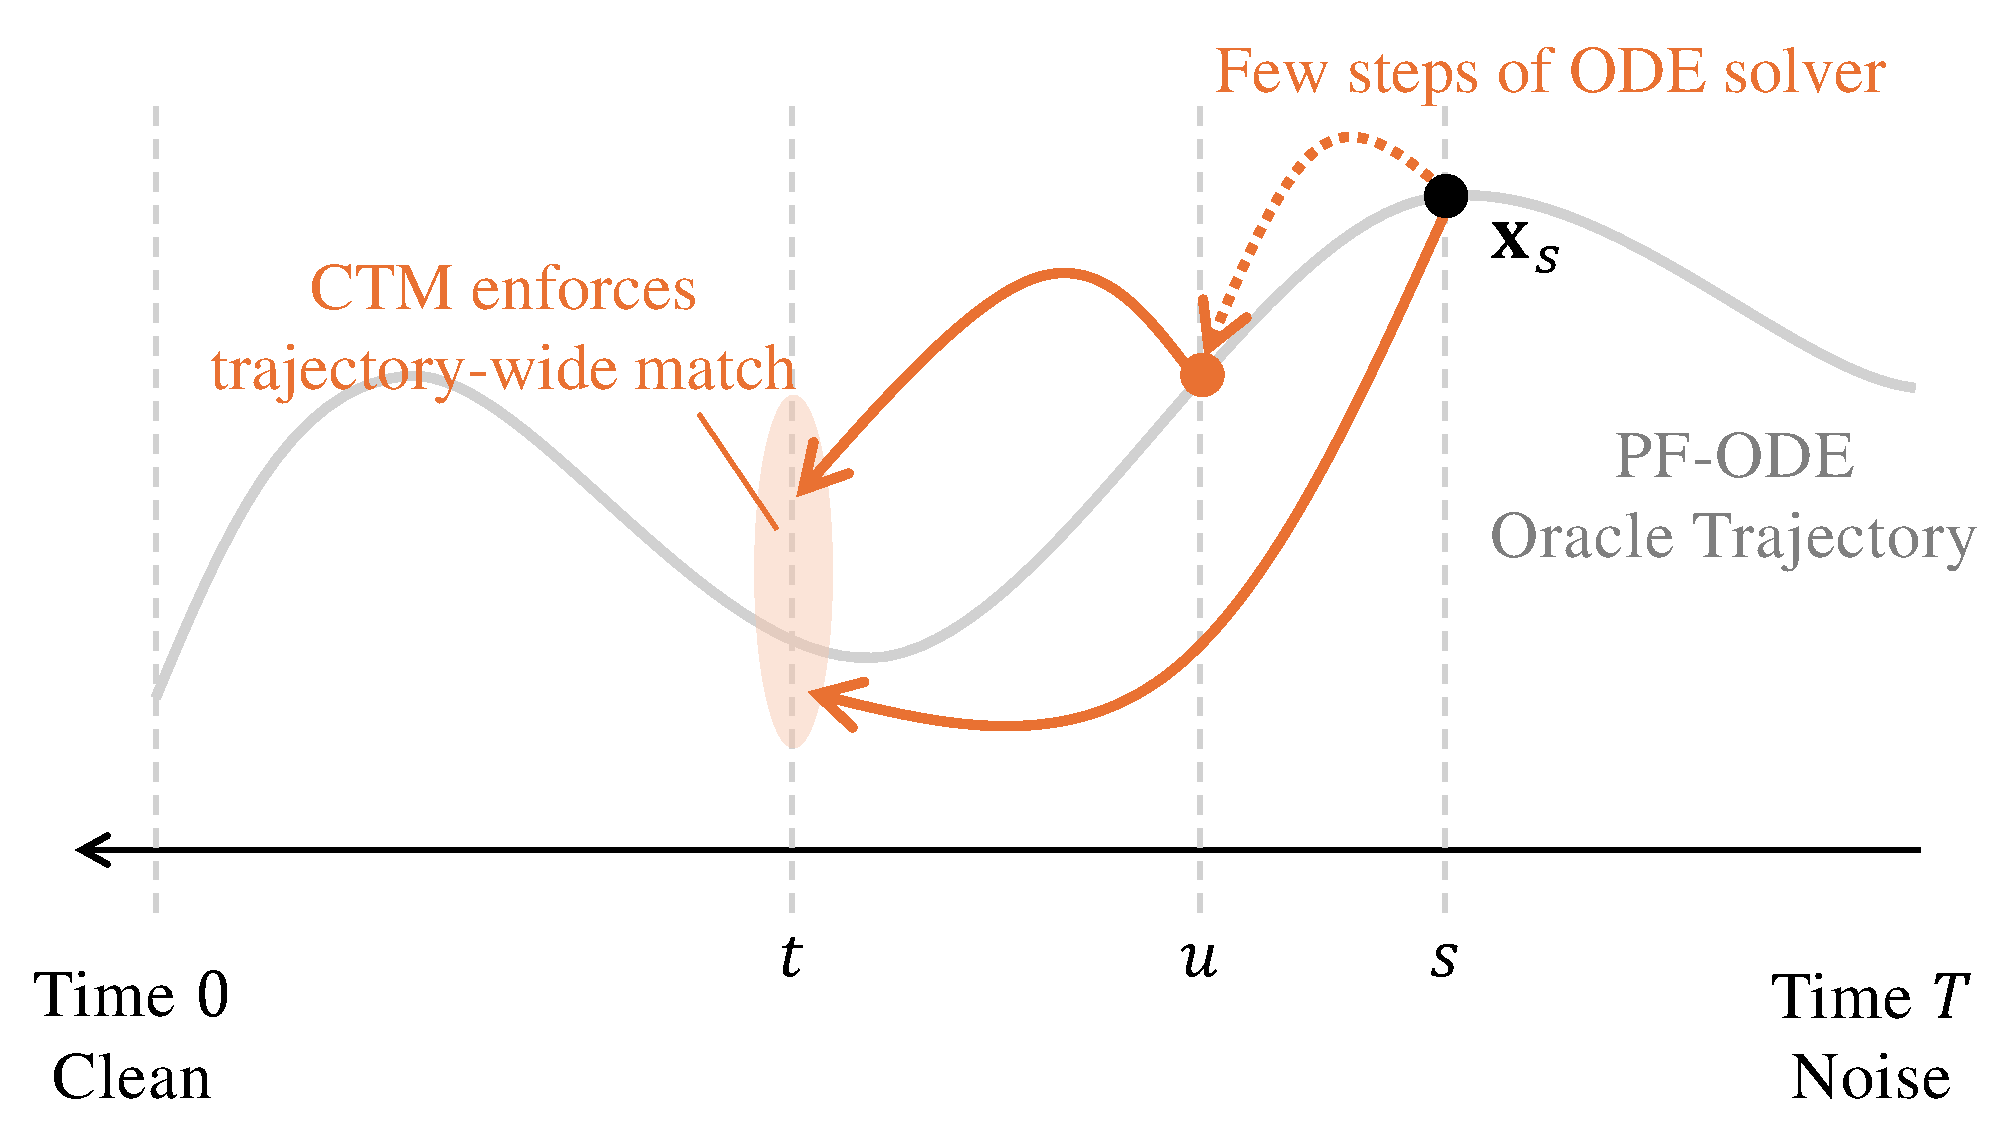
\includegraphics[width=0.9\linewidth]{Images/PartD/ctm-target.pdf}
    \caption{\textbfs{CTM 半群性质的图示。} 对于任何 $s \ge u \ge t$, CTM 强制执行
    $\rmG_{\btheta}(\rvx_s, s,  t)
\approx
\rmG_{\btheta^-} \big(\mathtt{Solver}_{s\to u}(\rvx_s), u ,  t\big)$，即短求解器段 $s \to u$ 随后是 CTM“跳转”到 $t$ 匹配直接CTM图 $s\to t$。求解器可以是预先训练的扩散或 CTM 的自诱导教师。 \figcredit{改编自 \citet{kim2023consistency}.}}
    \label{fig:ill_models}
\end{figure}

\subsection{CTM 中的辅助损失}\label{subsec:ctm-auxiliary}

（自）蒸馏可能表现不佳，因为它仅优化教师生成的目标，缺乏来自真实数据的直接监督。相比之下，CTM 可以自然地结合数据驱动的正则化器，例如通过降噪分数匹配和对抗性 (GAN) 项来增强其目标~\citep{goodfellow2014generative}，为了更好的学习流映射。 

\paragraph{扩散损耗的自然积分。}
扩散模型损失（更准确地说，条件流匹配损失；参见 \Cref{eq:fm-cfm})自然地集成到CTM中，并提供固定的回归目标，有利于流映射模型的学习。要看到这一点，请注意我们有
\[
\rvv^*(\rvx_s, s)
= \frac{\rvx_s - \rvg^*(\rvx_s, s, s)}{s},
\qquad 
\rvg^*(\rvx_s, s, s) \approx \rvg_{\btheta}(\rvx_s, s, s).
\]
这自然会通过以下方式引起速度参数化 $\rvg_{\btheta}$:
\[
\rvv_{\btheta}(\rvx_s, s)
:= \frac{1}{s}\bigl(\rvx_s - \rvg_{\btheta}(\rvx_s, s, s)\bigr).
\]
使用线性高斯路径
\[
\rvx_s = \alpha_s \rvx_0 + \sigma_s \beps,
\qquad
\rvx_0 \sim p_{\mathrm{data}}, 
\beps \sim \mathcal N(0, \mathbf I),
\]
扩散模型损失可以写为
\begin{align}\label{eq:ctm-dsm}
\mathcal L_{\mathrm{DM}}(\btheta)
&:= 
\E_{\rvx_0, \beps, s}
\Bigl[
w(s)
\bigl\|
 \rvv_{\btheta}(\rvx_s, s) - \left(\alpha_s' \rvx_0 + \sigma_s' \beps\right)
\bigr\|_2^2
\Bigr].
\end{align}



$\mathcal L_{\mathrm{DM}}$ 提高准确度 $t$ 接近 $s$ 通过明确监督沿轨迹的小跳跃。在这种制度下，因素 $1-\tfrac{t}{s}$ 在
\Cref{eq:ctm_para_1} 接近零，这会削弱梯度并减慢学习速度； $\mathcal L_{\mathrm{DM}}$ 提供更强的本地信号并稳定训练。从概念上讲， \Cref{eq:ctm-consist-distill,eq:ctm-consist-scratch} 强制轨迹匹配（零阶），同时 \Cref{eq:ctm-dsm} 强制斜率匹配（一阶）。

\paragraph{（选读）GAN 损失。}
虽然一致性和扩散模型损失提供了很强的回归信号，但它们可能会产生过于平滑的输出。因此，CTM 可以选择添加一个对抗性术语，通过将生成器分布与数据分布对齐来鼓励更清晰、更真实的样本。带鉴别器
$D_{\bm{\zeta}}$ 区分真实的 $\rvx_{0}\sim p_{\mathrm{data}}$ 来自生成 $\rvx_{\mathrm{est}}(\rvx_{s},s,t)$，目标是
\begin{align*} 
&\mathcal{L}_{\mathrm{GAN}}(\bm{\theta}, \bm{\zeta}) := \\ &\mathbb{E}_{\mathbf{x}_0} \big[\log D_{\bm{\zeta}}(\mathbf{x}_0)\big] + \mathbb{E}_{s \in [0, T]} \mathbb{E}_{t \in [0, s]} \mathbb{E}_{\mathbf{x}_0} \mathbb{E}_{\mathbf{x}_s \vert \mathbf{x}_0} \big[\log (1 - D_{\bm{\zeta}}( \mathbf{x}_{\mathrm{est}}(\mathbf{x}_s, s, t)))\big], \end{align*}
其中 $D_{\bm{\zeta}}$ 最大化并且 $\rmG_{\bm{\theta}}$ 已最小化。直观上，鉴别器充当自适应感知距离，鼓励现实细节。理论上，GAN 项驱动之间的分布匹配（詹森-香农散度） $p_{\mathrm{data}}$ 以及由以下引起的模型分布 $\rmG_{\bm{\theta}}$~\citep{goodfellow2014generative}，可以提高超出教师模型的保真度。

\paragraph{总体 CTM 目标。}
总之，CTM 将（自）蒸馏、扩散和 GAN 损失统一到一个训练框架中：
\begin{mdframed}
    \begin{align*}
\mathcal{L}_{\mathrm{CTM}}(\bm{\theta},\bm{\zeta})
:=  \mathcal{L}_{\mathrm{consist}}(\bm{\theta};  \bm{\phi}^\times/\bm{\theta}^-)
+ \lambda_{\mathrm{DM}} \mathcal{L}_{\mathrm{DM}}(\bm{\theta})
+ \lambda_{\mathrm{GAN}} \mathcal{L}_{\mathrm{GAN}}(\bm{\theta},\bm{\zeta}),
\end{align*}
\end{mdframed}
教师是外部预训练模型 $\bm{\phi}^\times$ 还是自引教师模型 $\bm{\theta}^-$。回归样式组件
$\mathcal{L}_{\mathrm{consist}}$ 和 $\mathcal{L}_{\mathrm{DM}}$ 充当强大的正则化器，而可选的 GAN 项可在不牺牲稳定性的情况下改善精细尺度细节~\citep{kim2024pagoda}.


\subsection{使用 CTM 进行灵活采样}
CTM学习通用流映射 $\bPsi_{s\to t}$ 对于任何 $s>t$，表示支持随时随地转换。此属性支持灵活的采样策略。例如，CTM建议 \emph{$\gamma$ 采样}，其中超参数 $\gamma$
控制生成过程中的随机性。此外，CTM 可以重用为扩散模型开发的标准推理技术，例如基于 ODE 的求解器和精确似然计算。接下来，我们固定一个离散时间网格进行采样 $T=\tau_0 > \tau_1 > \tau_2 > \cdots > \tau_{M}=0$.

\begin{algorithm}[H]
    \centering
    \caption{CTM 的 $\gamma$-采样}\label{alg:gamma}
    \begin{algorithmic}[1]
    \Require 经过训练的 CTM $\mathbf{G}_{\bm{\theta}^\times}$, $\gamma\in[0,1]$, $T=\tau_0>\tau_1 > \tau_2 > \cdots > \tau_{M}=0$.
    \State 从 $\mathbf{x}_{\tau_{0}}\sim p_{\mathrm{prior}}=\mathcal{N}(\bm{0}, T^2\rmI)$
        \For{$n=0$ 至 $M-1$}
        \State $\tilde{\tau}_{n+1}\leftarrow \sqrt{1-\gamma^{2}}\tau_{n+1}$
        \State 降噪 $\mathbf{x}_{\tilde{\tau}_{n+1}}\leftarrow \mathbf{G}_{\bm{\theta}^\times}(\mathbf{x}_{\tau_{n}},\tau_{n},\tilde{\tau}_{n+1})$
        \State 漫反射 $\mathbf{x}_{\tau_{n+1}}\leftarrow\mathbf{x}_{\tilde{\tau}_{n+1}}+\gamma \tau_{n+1}\bm{\epsilon}$，其中 $\bm{\epsilon}\sim\mathcal{N}(\bm{0}, \rmI)$
        \EndFor
        \Ensure  $\mathbf{x}_{\tau_{M}}$
    \end{algorithmic}
\end{algorithm}

\paragraph{方法论 $\gamma$-采样。}
CTM 的 $\gamma$-采样引入了一个统一的采样器系列，它是通过学习通用流映射模型自然产生的。它包含先前的方法，例如 CM 的多步采样（请参阅 \Cref{alg:cm_sampling}) 和时间步进式采样，其概念上类似于 ODE 求解器。参数 $\gamma$ 直接控制生成过程中语义变化的程度，使得 $\gamma$ 为不同的下游应用程序采样灵活的任务感知策略。





\begin{figure}[t]
    \centering
    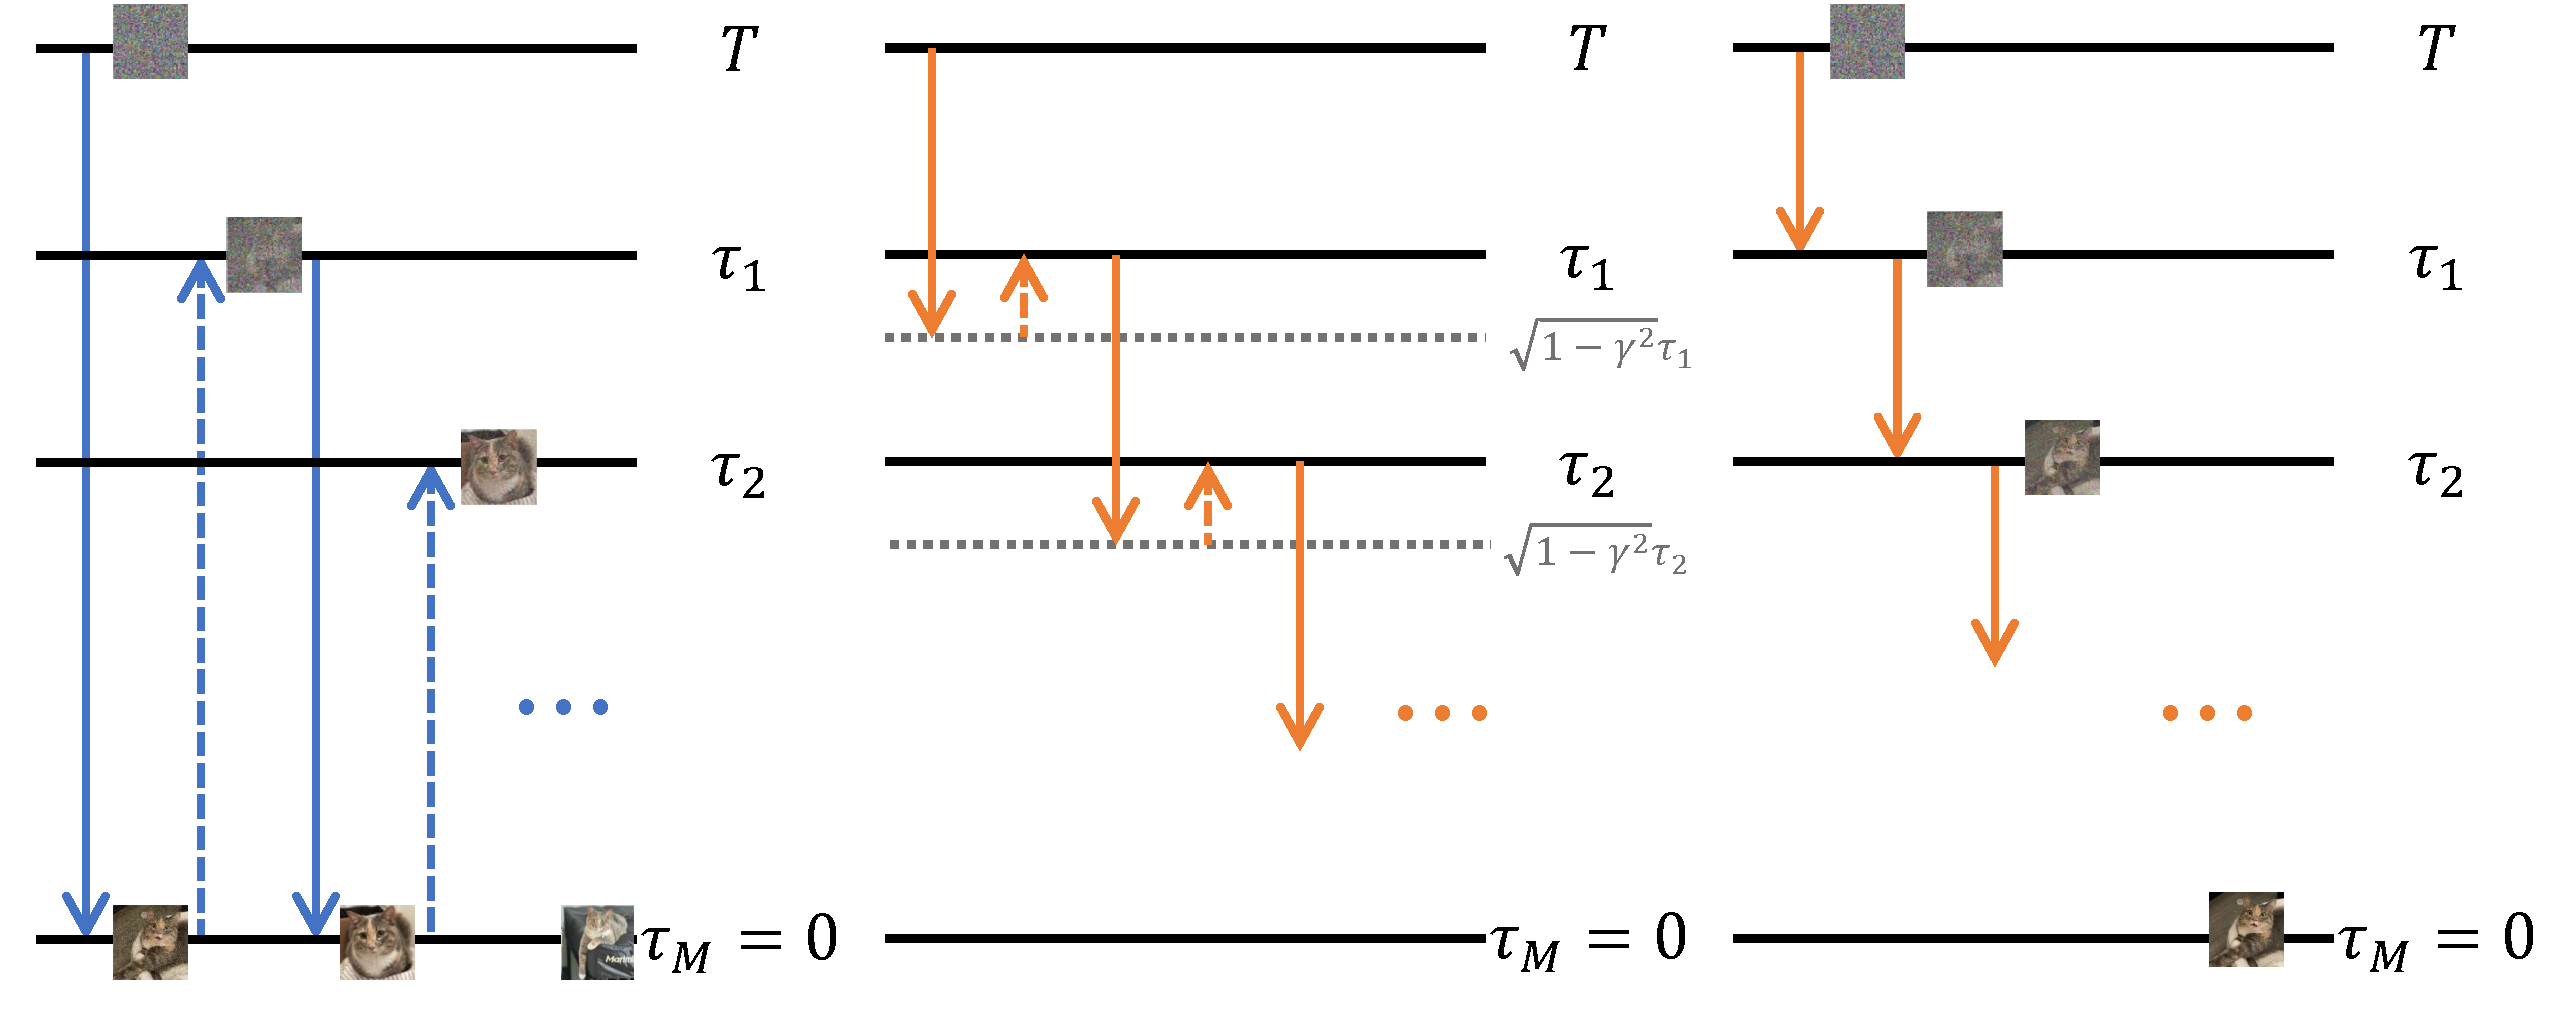
\includegraphics[width=\linewidth]{Images/PartD/ctm_gamma.pdf}
    \caption{\textbfs{插图 $\gamma$-采样变化 $\gamma$ 值。} 该过程在使用网络评估去噪和反向添加噪声之间交替，   $(\tau_{n}\xrightarrow{\text{Denoise}} \sqrt{1-\gamma^{2}}\tau_{n+1}\xrightarrow{\text{Noisify}} \tau_{n+1})_{n=0}^{M-1}$。最左边的面板说明 $\gamma=1$，对应于完全随机情况。最右边的面板显示 $\gamma=0$，对应于完全确定性情况。中间面板描绘了中间值 $\gamma\in(0,1)$，在这两个极端之间进行插值。 
\figcredit{改编自 \citet{kim2023consistency}.}}
    \label{fig:gamma_sampling}
\end{figure}


\begin{itemize}
\item \Cref{fig:gamma_sampling}-（左）：当 $\gamma=1$，与CM中引入的多步采样（即特殊的流映射 $\bPsi_{s\to 0}$)，它是完全随机的，当步数变化时会导致语义变化。

\item \Cref{fig:gamma_sampling}-（右）：当 $\gamma=0$，它简化为完全确定性时间步长，它估计 PF-ODE 的解轨迹。之间的一个关键区别 $\gamma$ 采样 $\gamma=0$ 与传统的基于时间步长 ODE 的采样相比，CTM 避免了数值求解器的离散化误差。

\item \Cref{fig:gamma_sampling}-(中): 当 $0 < \gamma < 1$, $\gamma$-通过允许在采样期间注入受控量的随机性，采样在两个极端之间进行插值。 
\end{itemize}
我们强调这一价值观 $\gamma\in[0,1)$ 需要一般流映射
$\bPsi_{s\to t}$，而特殊情况 $\gamma=1$ 简化为 CM 式多步采样，仅需要 $\bPsi_{s\to0}$.

\paragraph{分析 $\gamma$-采样。} CTM 根据经验观察到，一旦步数增加，CM 的多步采样质量就会下降 $M \geq 4$。为了解释这一现象，CTM分析了根本原因：当 $\gamma \neq 0$，每个神经“跳跃”都会引入一个小的不匹配，并且随着模型迭代地将状态映射到零时间，这些不匹配会累积。这种错误累积解释了为什么长时间的多步运行会表现不佳。我们在下面的命题中形式化了这个想法。

\proppp{（非正式）2步 $\gamma$-采样}{ctm-gamma}{
\label{th:sampling_agg_error_2_steps}
让 $\tau\in(0,T)$ 和 $\gamma \in [0,1]$。让 $p_{\bm{\theta}^{*},2}$ 表示从 $\gamma$-具有最佳 CTM 的采样器，遵循转换序列 $
    T\rightarrow\sqrt{1-\gamma^2}\tau\rightarrow \tau \rightarrow 0
$，从 $p_T$。然后
 \begin{align*}
    \mathcal D_{\mathrm{TV}}\big( p_{\mathrm{data}}, p_{\bm{\theta}^{*},2} \big)         = \mathcal{O}\left(\sqrt{T-\sqrt{1-\gamma^2}\tau+ \tau}  \right).
 \end{align*}
 在这里， $\mathcal{D}_{\mathrm{TV}}$ 表示分布之间的总变异（参见 \Cref{eq:f-div}).
}{
我们建议读者参考定理 8~\citet{kim2023consistency} 适用于采样步数为的一般情况 $M$. }
上述定理的结论可以总结如下：
\begin{itemize}
    \item \textbfs{当} $\gamma = 1$ （对应CM的多步采样）\textbfs{:} 该方法执行从 $\tau_n$ 至 $0$ 每一步 $n$。这会导致错误累积
    \begin{align*}
        \mathcal{O}\left(\sqrt{T + \tau_1 + \cdots + \tau_M}\right).
    \end{align*}
    
    \item \textbfs{当} $\gamma = 0$ （对应CTM的确定性多步采样）\textbfs{:} 消除了转换之间的这种时间重叠。这避免了错误累积并产生更严格的界限 $\mathcal{O}(\sqrt{T})$。根据经验，CTM $\gamma = 0$ 在采样速度和样本质量之间提供有利的权衡：增加采样步骤数可以提高生成质量，而不会引入不稳定。
\end{itemize}


\paragraph{CTM 支持扩散推理。} 由于CTM直接通过学习分数函数（或降噪器） $\rvg_{\bm{\theta}}$，由于其参数化 \Cref{eq:ctm_para_1}，它与最初为扩散模型开发的推理技术兼容。例如，我们可以计算精确似然（\Cref{subsec:sde-sample}) 或应用高级采样器，例如 DDIM 或 DPM (\Cref{ch:solvers}) 生成，通过使用 $\rvg_{\bm{\theta}}(\cdot, s, s)$.




\newpage

\section{\texorpdfstring{一般流映射：平均流}{一般流映射：平均流}}\label{sec:MF}


正如扩散模型承认许多等效的参数化和训练目标一样，通用流映射 $\bPsi_{s\to t}$ 也可以通过多种看似合理的方式来学习。在本节中，我们介绍 \emph{平均流} （MF）~\citep{geng2025mean}，后来通用流映射家族的代表 $\bPsi_{s\to t}$ 这说明了如何有效学习此类映射的另一种但有原则的观点。



\subsection{平均流的建模和训练}

与基于 EDM 框架构建的 CM 和 CTM 相比，MF 基于流匹配公式（$\alpha_t = 1-t$ 和 $\sigma_t  = t$ 用于 $t\in[0,1]$）。 MF 不是直接参数化流映射，而是学习 \emph{平均漂移}
在一段时间内 $[t,s]$ （与 $t<s$):
\[
\rvh_{\btheta}(\rvx_s, s, t)  \approx 
\rvh^*(\rvx_s, s, t) := \frac{1}{t-s}\int_s^t \rvv^*(\rvx_u,u) \diff u.
\]
对应的预言机损失为
\begin{align}\label{eq:mf-oracle}
\mathbb{E}_{t<s} \mathbb{E}_{\rvx_s\sim p_s}\Big[w(s) 
\|\rvh_{\btheta}(\rvx_s,s,t) - \rvh^*(\rvx_s,s,t)\|_2^2\Big].
\end{align}
特别是当 $s \to t$，损失函数简化为流匹配损失：
\begin{align}\label{eq:mf-to-fm}
    \mathbb{E}_{t} \mathbb{E}_{\rvx_t\sim p_t}\Big[w(t) 
\|\rvh_{\btheta}(\rvx_t,t,t) - \rvv^*(\rvx_t,t)\|_2^2\Big],
\end{align}
学习瞬时速度。我们稍后会看到 \Cref{subsec:equivalence-ctm-mf} MF 与总体目标保持一致 \Cref{eq:general-cm-loss:rep}，但从不同（虽然等效）的角度来处理它。由于oracle回归目标 $\rvh^*(\rvx_s,s,t)$ 一般不承认封闭形式，MF通过利用微分获得的恒等式来构造代理
\[
(t-s)\,\rvh^*(\rvx_s,s,t) = \int_s^t \rvv^*(\rvx_u,u)\,\diff u
\]
相对于 $s$。这产生了 \emph{MF恒等式}:
\begin{align}\label{eq:mf-identity}
\begin{aligned}
    \rvh^*(\rvx_s,s,t)
&= \rvv^*(\rvx_s,s) - (s-t) \tfrac{\diff}{\diff s}\rvh^*(\rvx_s,s,t) \\
&= \rvv^*(\rvx_s,s) - (s-t)\Big[(\partial_{\rvx}\rvh^*)(\rvx_s,s,t) \rvv^*(\rvx_s,s) 
+ \partial_s \rvh^*(\rvx_s,s,t)\Big],
\end{aligned}
\end{align}
第二行将链式法则与 
\[
\frac{\diff}{\diff s}\rvx_s = \rvv^*(\rvx_s,s).
\]

受此恒等式的激励，MF 用停止梯度代理替代了棘手的预言，从而实现了实际的训练目标
\begin{mdframed}
\begin{align}\label{eq:mf-practice}
    \mathcal{L}_{\mathrm{MF}}(\btheta)
:= \mathbb{E}_{t<s} \mathbb{E}_{\rvx_s\sim p_s}\Big[w(s)\,
\|\rvh_{\btheta}(\rvx_s,s,t) - \rvh_{\btheta^-}^{\mathrm{tgt}}(\rvx_s,s,t)\|_2^2\Big],
\end{align}
\end{mdframed}
其中回归目标定义为
\begin{align*}
    \rvh_{\btheta^-}^{\mathrm{tgt}}&(\rvx_s,s,t)
:= \\ &\rvv^*(\rvx_s,s) - (s-t)\Big[\underbrace{(\partial_{\rvx}\rvh_{\btheta^-})(\rvx_s,s,t) \rvv^*(\rvx_s,s)
+ \partial_s \rvh_{\btheta^-}(\rvx_s,s,t)}_{\mathrm{JVP}}\Big].
\end{align*}

在实践中，预言机速度 $\rvv^*$ 无法以封闭形式计算，必须进行近似计算。有两种常见的策略可用：依靠预先训练的扩散模型（\emph{蒸馏}) 或根据数据构建直接估计器 (\emph{从头开始训练}）。无论选择如何，最终都需要计算一个
\emph{雅可比矩阵与向量的乘积}  目标网络的（JVP）
$\rvh_{\btheta^-}$:
\[ 
\left[\partial_\rvx \rvh_{\btheta^-}, \partial_s \rvh_{\btheta^-}, \partial_t \rvh_{\btheta^-}\right]^\top \cdot \left[\rvv^*, 1, 0\right]
\]


\paragraph{蒸馏。}
使用具有流匹配主干的预训练扩散模型，
$\rvv_{\bphi^\times} \approx \rvv^*$.

\paragraph{从头开始训练。}
使用一点条件速度 $\alpha_s'\rvx_0 + \sigma_s'\beps$，从前向噪声注入获得 $\rvx_s=\alpha_s\rvx_0+\sigma_s\beps$ 与
$\beps\sim\mathcal N(\bm{0},\rmI)$。这给出了液位瞬时漂移的无偏单样本估计 $s$ 配对时评估 $(\rvx_0,\beps)$.



\subsection{平均流采样}
曾经是MF $\rvh_{\btheta^\times}$ 经过训练，它自然恢复了流映射的代理。对于任何起点 $\rvx_s$，映射来自 $s$ 到 $t$ （大约）由下式给出
\[
\bPsi_{s\to t}(\rvx_s) = \rvx_s + (t-s)\,\rvh^*(\rvx_s,s,t)
  \approx   \rvx_s + (t-s)\,\rvh_{\btheta^\times}(\rvx_s,s,t).
\]

这可以实现单步和多步采样。例如，绘图
$\rvx_T\sim p_{\mathrm{prior}}$，一步生成干净样本是
\[
\rvx_0  \leftarrow  \rvx_T - T\,\rvh_{\btheta^\times}(\rvx_T,T,0).
\]

或者，可以通过准备时间网格并按顺序应用映射来执行多步生成，与 CTM 中使用的时间步长方式相同。由于MF学习了通用的流映射，因此它还支持 $\gamma$-如 CTM 中的采样，其中可控超参数 $\gamma$ 将随机性注入采样过程。

\subsection{CTM与MF的关系}\label{subsec:equivalence-ctm-mf}
乍一看，CTM 和 MF 似乎无关。  
事实上，两者都提供相同预言流的不同参数化
映射$\bPsi_{s\to t}$，及其对应的平方预言回归
误差与时间相关的权重~\citep{hu2025cmt}相关。

\paragraph{参数化关系.}
两种方法在相同的总体框架下运行，但以不同的方式表示学习的功能。  
流映射可以等效地写为
\begin{align*}
\bPsi_{s\to t}(\rvx_s)
& = \rvx_s + \int_s^t \rvv^*(\rvx_u, u)\diff u \\
&= \frac{t}{s}\rvx_s
   + \frac{s-t}{s}\underbrace{\Bigg[\rvx_s + \frac{s}{s-t}\int_s^t \rvv^*(\rvx_u,u)\,\diff u\Bigg]}_{\approx\,\rvg_\btheta} \\
&= \rvx_s + (t-s)\underbrace{\Bigg[\frac{1}{t-s}\int_s^t \rvv^*(\rvx_u,u)\,\diff u\Bigg]}_{\approx\,\rvh_\btheta}.
\end{align*}
这里，第一个是流映射的定义，第二个形式通过$\rvg_\btheta$突出显示CTM参数化（参见\Cref{eq:ctm-g-oracle,eq:ctm_para_1}），而最后一个形式通过$\rvh_\btheta$突出显示MF参数化。  


\paragraph{训练损失的关系。} 根据上述对预言机流映射$\bPsi_{s\to t}$在CTM参数化方面的重新解释 
\[
\rvg_\btheta(\rvx_s,s,t) \approx \rvg^*(\rvx_s,s,t):=\rvx_s + \frac{s}{s-t}\int_s^t \rvv^*(\rvx_u,u) \diff u
\]
 和 MF 参数化 
\[
\rvh_\btheta(\rvx_s,s,t) \approx \rvh^*(\rvx_s,s,t):=\frac{1}{t-s}\int_s^t \rvv^*(\rvx_u,u) \diff u,
\] 
我们现在证明 CTM 和 MF 的训练损失实际上是相等的。


考虑关系
\[
\rvg_\btheta(\rvx_s,s,t) := \rvx_s - s \rvh_\btheta(\rvx_s,s,t),
\]
以$d(\rvx,\rvy):=\|\rvx-\rvy\|^2$为例。代入 \Cref{eq:general-cm-loss:rep} 并将 $\rmG_\btheta$ 视为 CTM 的流映射参数化 (\Cref{eq:ctm_para_1}) 给出
\begin{align} &~d\big(\rmG_\btheta(\rvx_s,s,t), \bPsi_{s\to t}(\rvx_s)\big) \notag \\ = &~\norm{\rmG_\btheta(\rvx_s,s,t) - \bPsi_{s\to t}(\rvx_s)}^2 \notag \\ = &~\norm{\left(\frac{t}{s}\rvx_s + \frac{s-t}{s} \rvg_\btheta(\rvx_s,s,t)\right)-\left(\frac{t}{s}\rvx_s + \frac{s-t}{s}\Big[\rvx_s + \frac{s}{s-t}\int_s^t \rvv^*(\rvx_u,u) \diff u\Big]\right)}^2 \notag \\ = &~\left(\frac{s-t}{s}\right)^2\norm{\rvg_\btheta(\rvx_s,s,t)-\left(\rvx_s + \frac{s}{s-t}\int_s^t \rvv^*(\rvx_u,u) \diff u\right)}^2 \label{eq:g-para} \\ = &~\left(\frac{s-t}{s}\right)^2\norm{\left(\rvx_s - s \rvh_\btheta(\rvx_s,s,t)\right)-\left(\rvx_s + \frac{s}{s-t}\int_s^t \rvv^*(\rvx_u,u) \diff u\right)}^2 \notag \\ = &~\left(\frac{s-t}{s}\right)^2\norm{\left(\rvx_s - s \rvh_\btheta(\rvx_s,s,t)\right)-\left(\rvx_s + \frac{s}{s-t}\int_s^t \rvv^*(\rvx_u,u) \diff u\right)}^2 \notag \\ = &~\left(s-t\right)^2\norm{ \rvh_\btheta(\rvx_s,s,t)- \left(\frac{1}{t-s}\int_s^t \rvv^*(\rvx_u,u)\diff u \right)}^2 \label{eq:h-para} \end{align}
因此，
\begin{align*} 
\frac{1}{s^2} \Bigg\|\rvg_\btheta(\rvx_s,s,t)-\rvg^*(\rvx_s,s,t) \Bigg\|^2 = \Bigg\|\rvh_\btheta(\rvx_s,s,t)-\rvh^*(\rvx_s,s,t) \Bigg\|^2. 
\end{align*}
抛开用于学习流映射的特定算法不谈，CTM 和 MF 损失具有相同的数学形式，仅加权函数不同。此外，在任一情况下设置 $t=0$ 都会恢复 CM 设置 ($\bPsi_{s\to 0}$)，其中
每个状态都直接映射到干净的数据。

\paragraph{实践中的辅助损失.}
在CTM中，使用\Cref{eq:ctm-consist-scratch}中的一致性损失与其自定义的\Cref{eq:ctm-dsm}中的扩散模型损失一起进行训练。 MF 中也采用了类似的策略。如\Cref{eq:mf-to-fm}所示，当$s \to t$时，MF损失降低至标准流匹配目标。实际中，MF控制的是$s \neq t$与$s = t$的配对比例；因此，整体优化变成了\Cref{eq:mf-practice}中的MF目标和\Cref{eq:mf-to-fm}中的流匹配目标的混合。 

两种参数化都能够提供从扩散模型训练（通过固定回归目标学习瞬时速度）到流映射学习（采用停止梯度伪回归目标）的平滑过渡。\paragraph{CTM和MF参数化实现灵活推理。}
CTM ($\rmG_\btheta(\rvx_s,s,t)$) 和 MF ($\rvh_\btheta(\rvx_s,s,t)$) 都旨在近似底层流映射 $\bPsi_{s\to t}$：
\[
\rmG_\btheta(\rvx_s,s,t)\approx\bPsi_{s\to t},\quad  \text{and}
\quad 
\rvx_s+(t-s)\rvh_\btheta(\rvx_s,s,t)\approx\bPsi_{s\to t}.
\]
由于这两个模型都学习任意两个时间步之间的显式映射，因此它们自然支持 CTM 的 $\gamma$ 采样，并与最初为扩散模型开发的推理技术保持兼容，例如引导 (\Cref{ch:guidance})、精确似然计算 (\Cref{eq:score-sde-likelihood}) 和使用高阶求解器的加速采样 (\Cref{ch:solvers})。 
这种兼容性的出现是因为它们的参数化恢复了无限小极限 $t\to s$ 中的瞬时扩散漂移：
\[
\rvg^*(\rvx_s,s,s)=\rvx_s-s\,\rvv^*(\rvx_s,s),
\quad  \text{and}
\quad 
\rvh^*(\rvx_s,s,s)=\rvv^*(\rvx_s,s).
\]
专门的流映射配方 $\bPsi_{s\to0}$ 不具有此属性，例如 CM 系列中的配方。因此，CTM 和 MF 都可以被视为灵活且通用的流映射公式，将基于扩散的推理推广到直接时间到时间映射。




\paragraph{结论.}



CTM 和 MF 之间的关系类似于
扩散模型的不同参数化
(\Cref{sec:equivalent-parametrizations})：在预言机级别，它们编码
相同的底层流映射。根据平方误差回归和参数化
上述关系中，它们的预言机回归误差仅因已知的差异而不同
与时间相关的缩放。然而，他们的实际训练目标仍然是
不同是因为他们使用不同的替代目标和优化
程序。

尽管 CTM 和 MF 以这种方式相关，但它们在概念和算法上在如何学习目标方面有所不同。 CTM 目标以“整体”形式定义，因为它直接作用于流映射。另一方面，MF 目标以“微分”形式定义，因为它依赖于流映射的有限差分。由于积分形式的目标无法直接处理，因此 CTM 必须在训练期间求解 ODE。相比之下，MF 利用 MF 恒等式（参见 \Cref{eq:mf-identity}）以差分形式构造一个易于处理的目标。这种关系类似于基于能量的方法和基于分数的方法之间的关系：前者学习概率密度本身（以积分形式），而后者匹配该密度的梯度（以微分形式）。在实践中，由于损失权重、网络架构和优化动态等因素，CTM 和 MF 的表现可能有所不同，这可能导致一种方法在某些条件下比另一种方法表现更好。

这种观点表明 CTM 和 MF 并不是唯一可行的配方。流映射的其他参数化也可以实现高效稳定的训练，有可能产生新的独立生成模型。探索这些替代方案可能会进一步丰富扩散模型及其流映射扩展的前景，从而突破少步生成的界限。

\clearpage
\newpage

\section{结束语}\label{sec:ch11_cr}

最后一章使我们的探索完整了：从缓慢的迭代扩散采样器到快速的几步生成器（从头开始学习）。本章中的方法背后的共同的学习对象是中介绍的oracle流映射 \Cref{eq:general-cm-loss:rep}:
\[
\bPsi_{s\to t}(\rvx_s)
=
\rvx_s+\int_s^t \rvv^*(\rvx_\tau,\tau)\,\diff \tau.
\]
学习这张映射可以通过一次或几次学习的跳跃来替换许多小的数值更新。此时，退出各个算法是很有用的。知识蒸馏（\Cref{sec:distillation-prologue})，渐进式蒸馏 (\Cref{sec:PD}), CM (\Cref{sec:discrete-cm}), CTM (\Cref{sec:CTM}) 和 MF (\Cref{sec:MF}) 是通过不同的训练结构引入的，但它们都显式或隐式地利用相同的 ODE 解映射结构。流映射本身是微分方程和动力系统中的经典对象，与连续介质和流体力学中基于粒子和基于场的描述密切相关；看到
\Cref{eq:flow-map-def} 以及周围的历史讨论。在这里，我们使用同一 ODE 流程的三种经典描述，即 \emph{半群}, \emph{拉格朗日}, 和 \emph{欧拉} 观点，作为上面开发的现代学习方法的组织镜头
\footnote{在现代生成建模中， \citet{boffi2024flow} 汇集 PD、CM、CTM 和 MF 中已经出现的结构思想，并使用它们以通用语言描述扩散 PF-ODE 流映射的学习。因此，主要成分很大程度上来自这些现有的工作。我们在这部分的演示和插图也来自于以下的阐述： \citet{dieleman2026flowmaps}.}


\paragraph{半群视图：分头旅行。}
如中所述 \Cref{eq:semi-group}，有限步恒等式为
\[
\bPsi_{u\to t}\big(\bPsi_{s\to u}(\rvx_s)\big)
=
\bPsi_{s\to t}(\rvx_s).
\]
如图所示 \Cref{fig:semigroup}，直觉上和沿着固定路线行驶是一样的：从 $s$ 至
$u$ 然后从 $u$ 至 $t$ 降落在与直接从
$s$ 至 $t$。在这个视图中，KD 学习了完整的转变 $\bPsi_{T\to0}$，PD将两个相邻的教师步压缩为一个学生步，CM学习特殊的随时清理图 $\bPsi_{s\to0}$，和CTM将相同的构成原理扩展到通用映射 $\bPsi_{s\to t}$.

\begin{figure}[t]
    \centering

    \begin{subfigure}[t]{0.485\textwidth}
        \centering
        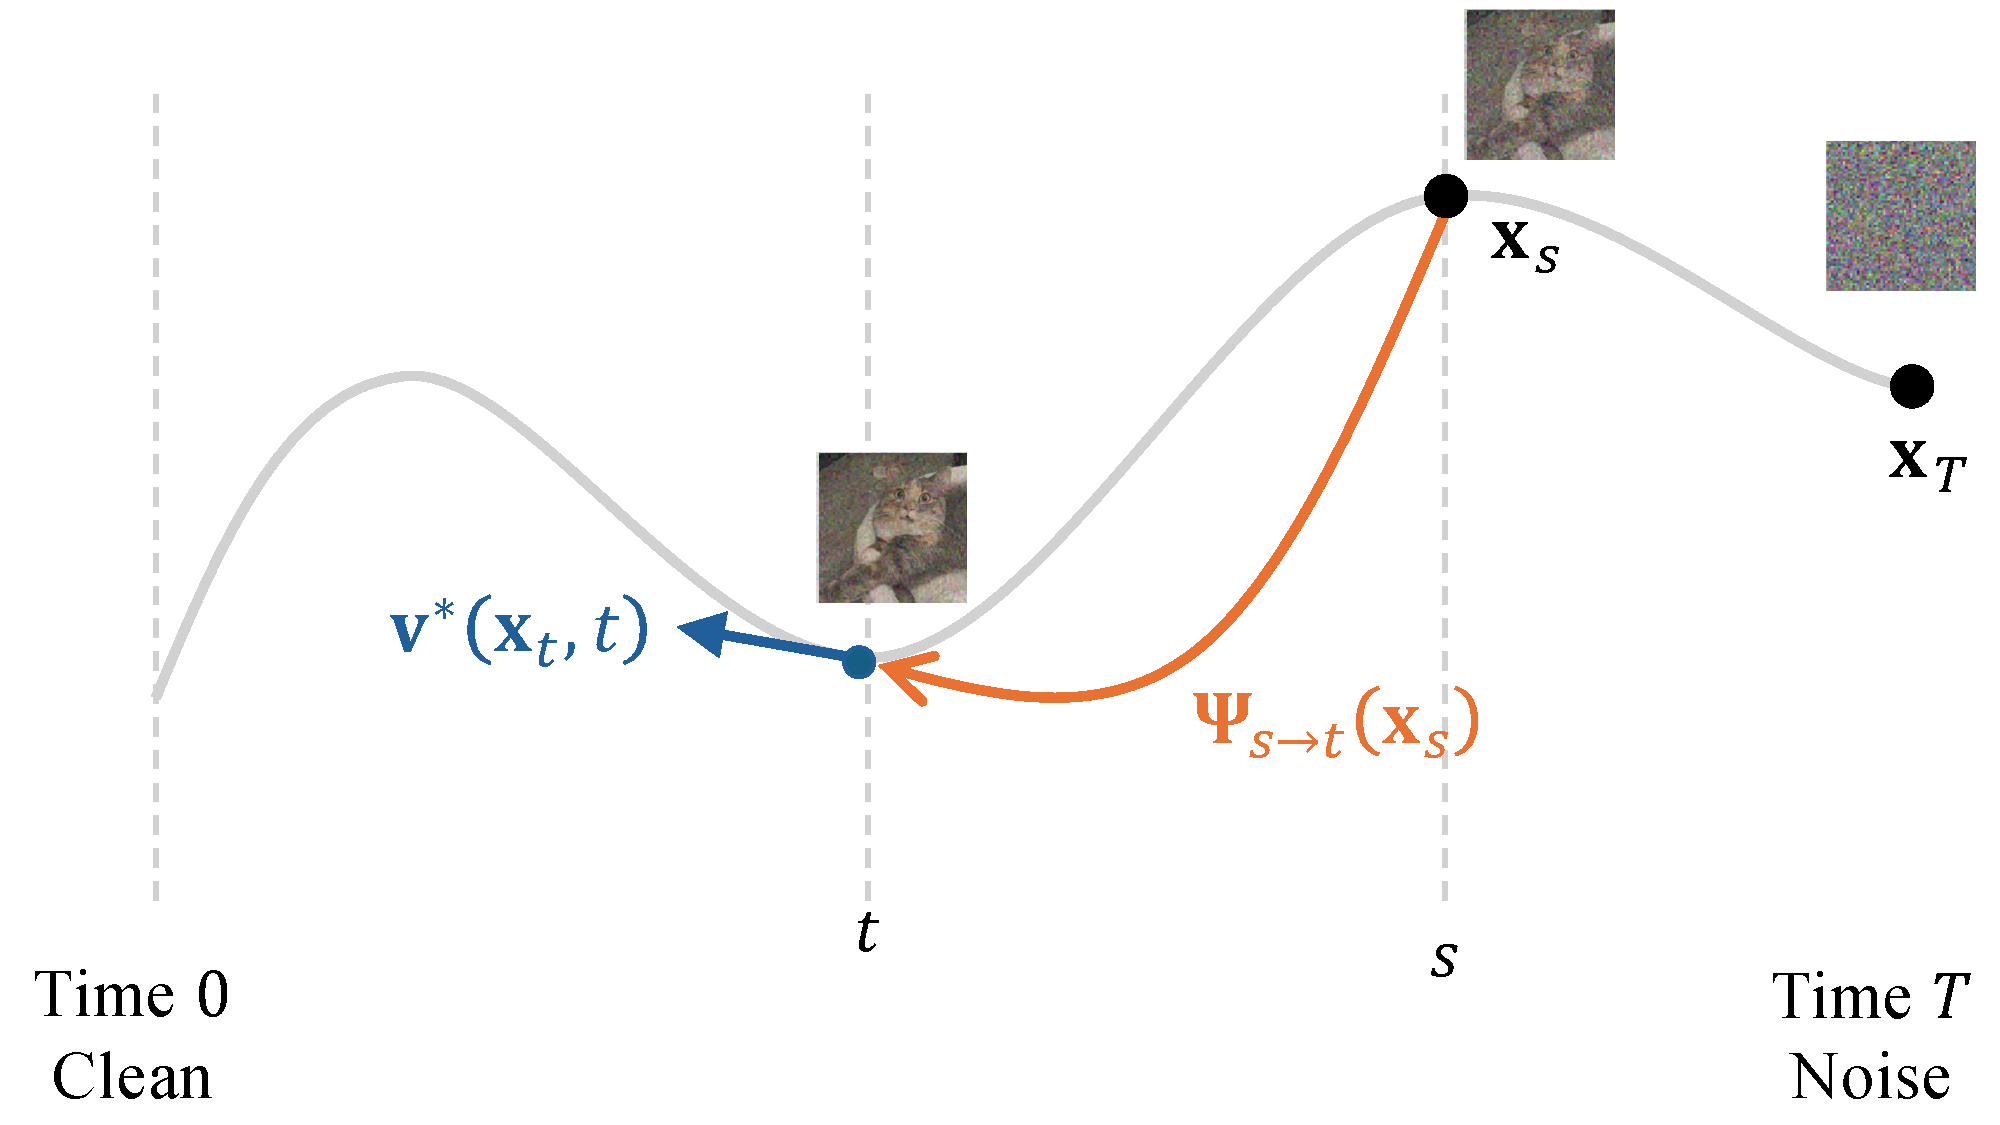
\includegraphics[width=\linewidth]{Images/PartD/lagrangian-1.pdf}
        \caption{基准结束时间 $t$.}
        \label{fig:lagrangian-base}
    \end{subfigure}
    \hfill
    \begin{subfigure}[t]{0.485\textwidth}
        \centering
        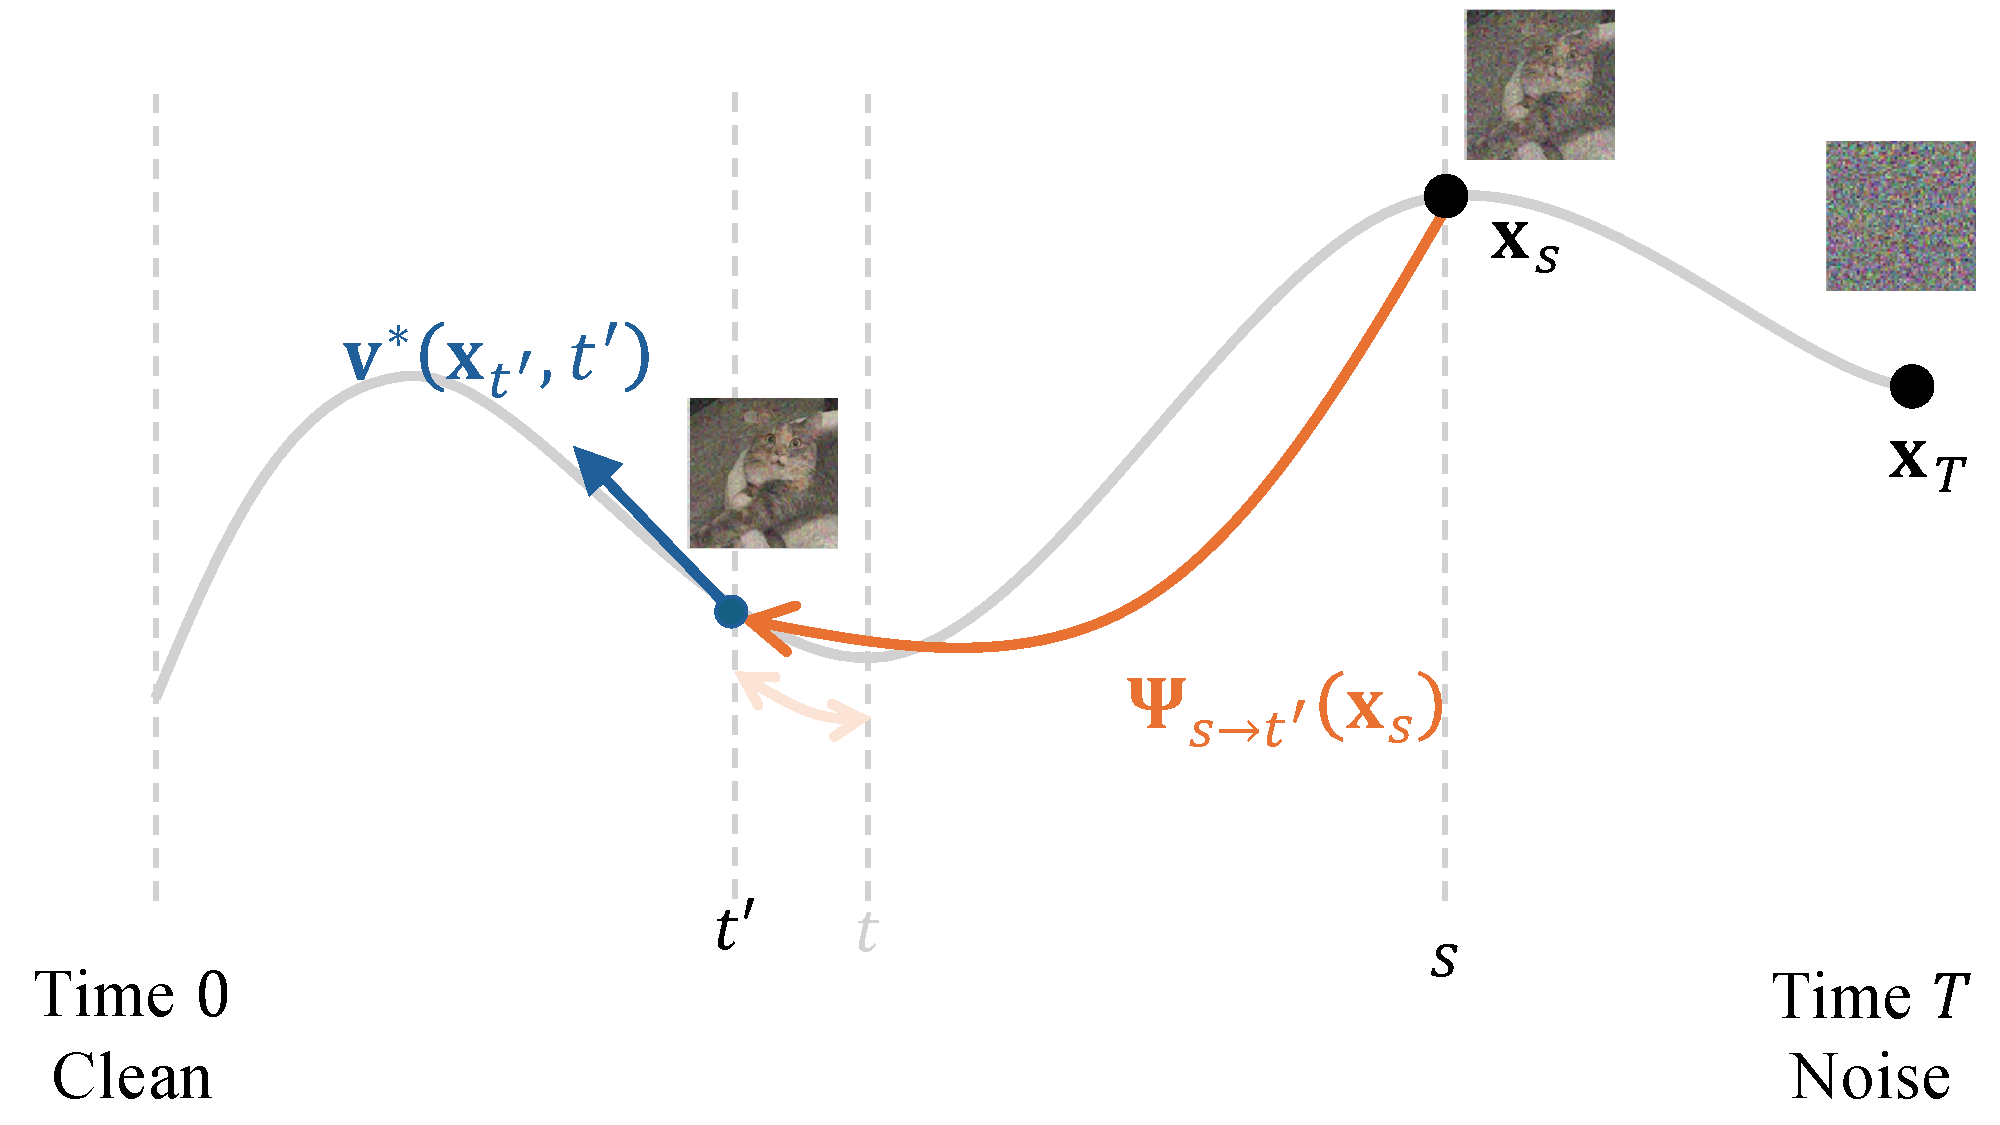
\includegraphics[width=\linewidth]{Images/PartD/lagrangian-2.pdf}
        \caption{移动结束时间 $t'$.}
        \label{fig:lagrangian-moved}
    \end{subfigure}\caption{\textbfs{流映射的拉格朗日一致性。}
    起始状态-时间对 $(\rvx_s,s)$ 固定，结束时间从 $t$ 移至
    $t'$。流映射的输出沿着相同的 PF-ODE 轨迹移动，并且
    其无穷小的变化等于 ODE 速度：
    $\partial_t \bPsi_{s\to t}(\rvx_s)
    = \rvv^*(\bPsi_{s\to t}(\rvx_s),t)$.}
    \figcredit{改编自\citet{dieleman2026flowmaps}.}
    \label{fig:lagrangian-consistency}
\end{figure}

\paragraph{拉格朗日视图：移动终点。}
修复起始状态-时间对 $(\rvx_s,s)$ 并改变结束时间
$t$。然后终点沿着相同的轨迹移动：
\[
\partial_t \bPsi_{s\to t}(\rvx_s)
=
\rvv^*(\bPsi_{s\to t}(\rvx_s),t).
\]
“拉格朗日”这个名字遵循经典粒子观点：我们
随着结束时间的变化，沿着轨迹跟踪结束点。
无限小地，终点以局部 ODE 速度移动
当时评价的。

\paragraph{Eulerian 视图：移动起点。}
固定结束时间$t$，并沿相同轨迹滑动起点。
时间 $t$ 的结束点保持固定：
\[
\frac{\diff}{\diff s}\bPsi_{s\to t}(\rvx_s)=0.
\]
自 $\frac{\diff}{\diff s}\rvx_s=\rvv^*(\rvx_s,s)$ 起，链式法则给出
\[
\partial_s\bPsi_{s\to t}(\rvx_s)
+
\big(\partial_{\rvx}\bPsi_{s\to t}\big)(\rvx_s)\rvv^*(\rvx_s,s)
=
0.
\]
“欧拉”一词引用了经典的基于场的观点：这里，结束时间 $t$
是固定的，而起始状态-时间对 $(\rvx_s,s)$ 沿着
相同的 ODE 轨迹；因此，时间 $t$ 的结束点保持不变。对于 CM，结束时间固定为 $t=0$，因此结束点是干净的样本：
\[
    \rvf^*(\rvx_s,s)=\bPsi_{s\to0}(\rvx_s).
\]
因此，\Cref{eq:conti-ct-motivation} 是启动时间一致性条件
对于\Cref{sec:discrete-cm,sec:conti-cm}中研究的特殊流映射。



这个观点也概括了CTM和MF之间的关系
\Cref{subsec:equivalence-ctm-mf}。  两者近似相同的路径积分
\[
\bPsi_{s\to t}(\rvx_s)
=
\rvx_s+\int_s^t\rvv^*(\rvx_\tau,\tau)\,\diff\tau,
\]
但暴露不同的可训练代理。  CTM通过位移式表示终点
参数化，而 MF 表示通过
平均漂移
\[
\rvh^*(\rvx_s,s,t)
=
\frac{1}{t-s}\int_s^t\rvv^*(\rvx_\tau,\tau)\,\diff\tau.
\]
替代
\[
\bPsi_{s\to t}(\rvx_s)=\rvx_s+(t-s)\rvh^*(\rvx_s,s,t)
\]
转化为欧拉起始时间恒等式
\[
\rvh^*(\rvx_s,s,t)
=
\rvv^*(\rvx_s,s)
-
(s-t)
\left[
\partial_s\rvh^*(\rvx_s,s,t)
+
(\partial_{\rvx}\rvh^*)(\rvx_s,s,t)\rvv^*(\rvx_s,s)
\right].
\]
这是基本的平均流恒等式：较长时间间隔内的平均漂移为
起点处的瞬时漂移，通过平均漂移进行校正
随着起点沿着相同的轨迹滑动而变化。

\begin{figure}[t]
    \centering

    \begin{subfigure}[t]{0.485\textwidth}
        \centering
        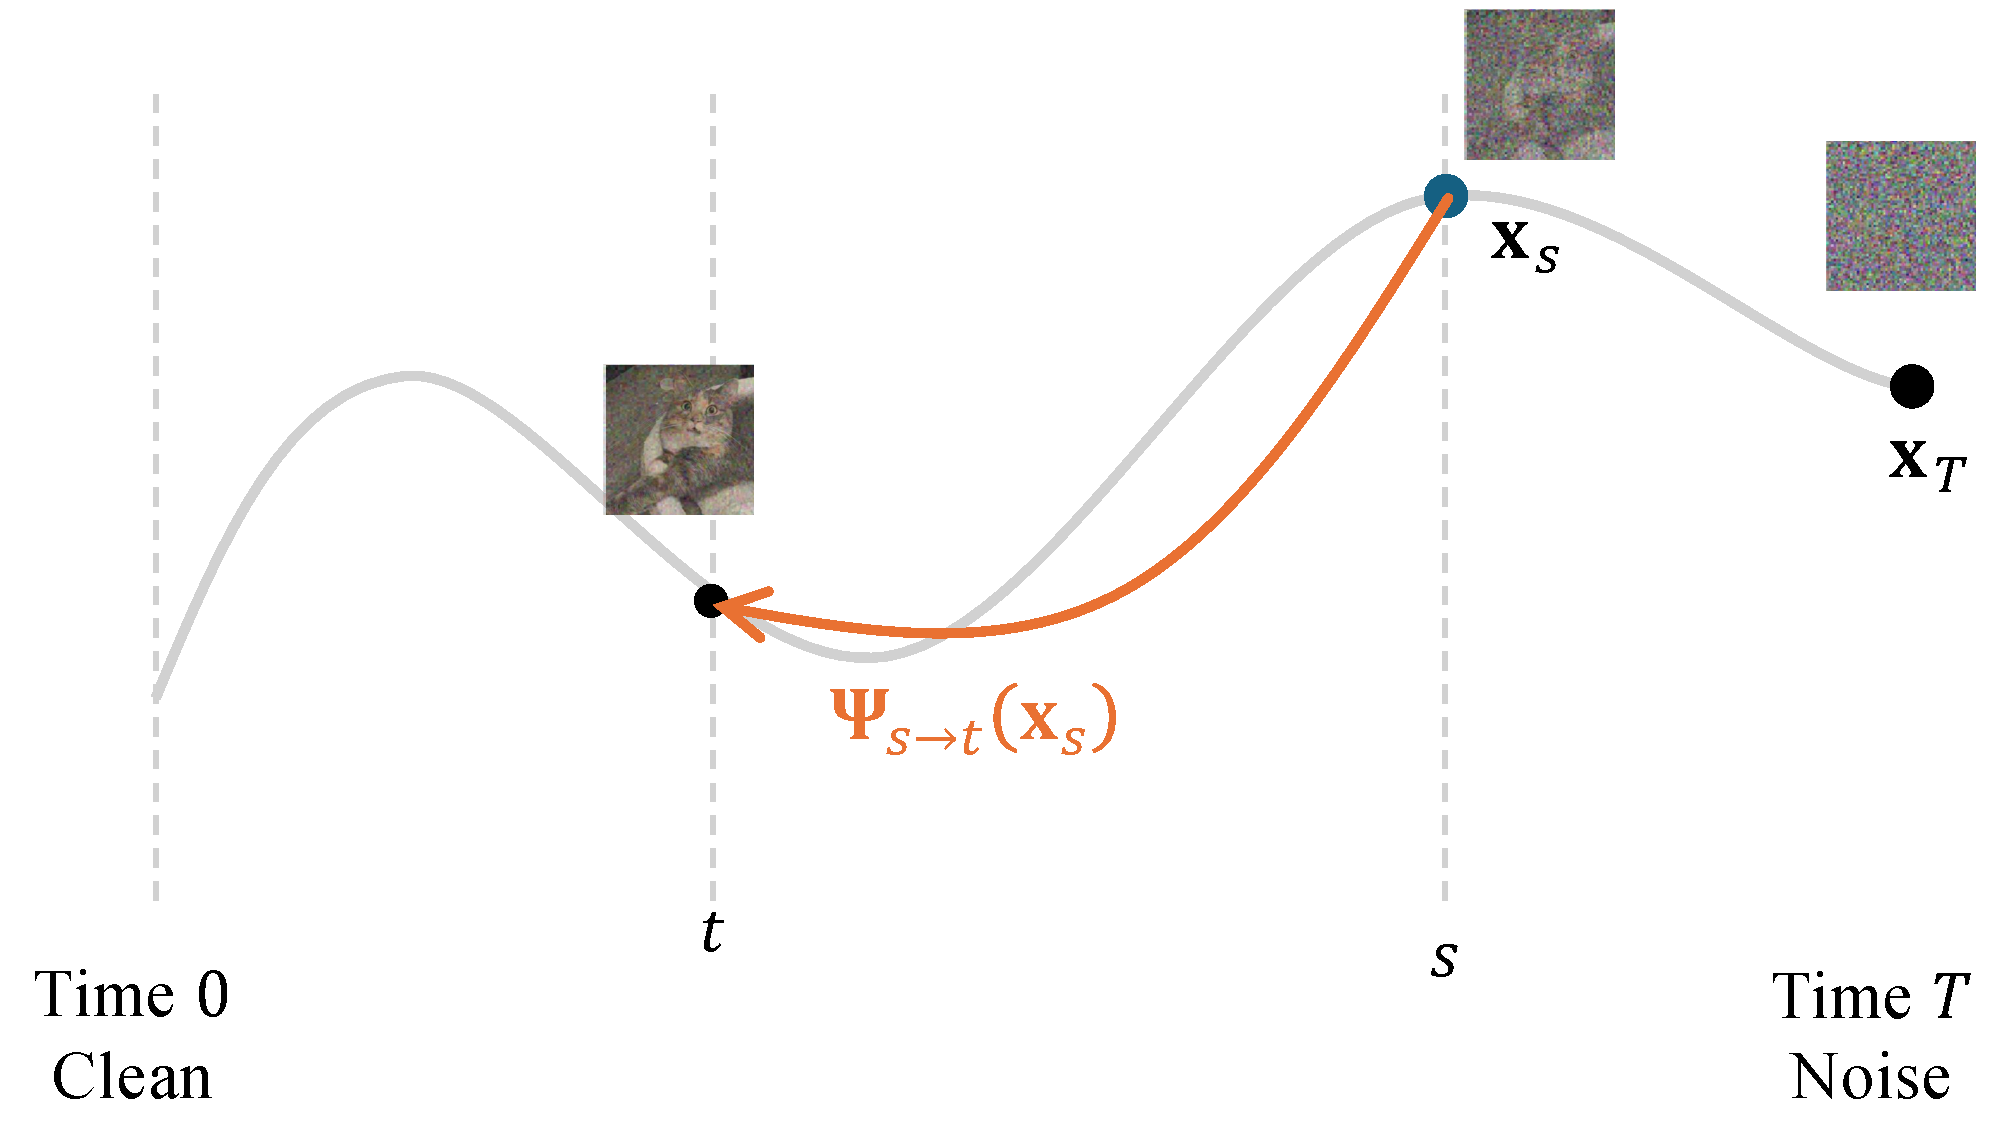
\includegraphics[width=\linewidth]{Images/PartD/eulerian-1.pdf}
        \caption{基准启动时间 $s$.}
        \label{fig:eulerian-base}
    \end{subfigure}
    \hfill
    \begin{subfigure}[t]{0.485\textwidth}
        \centering
        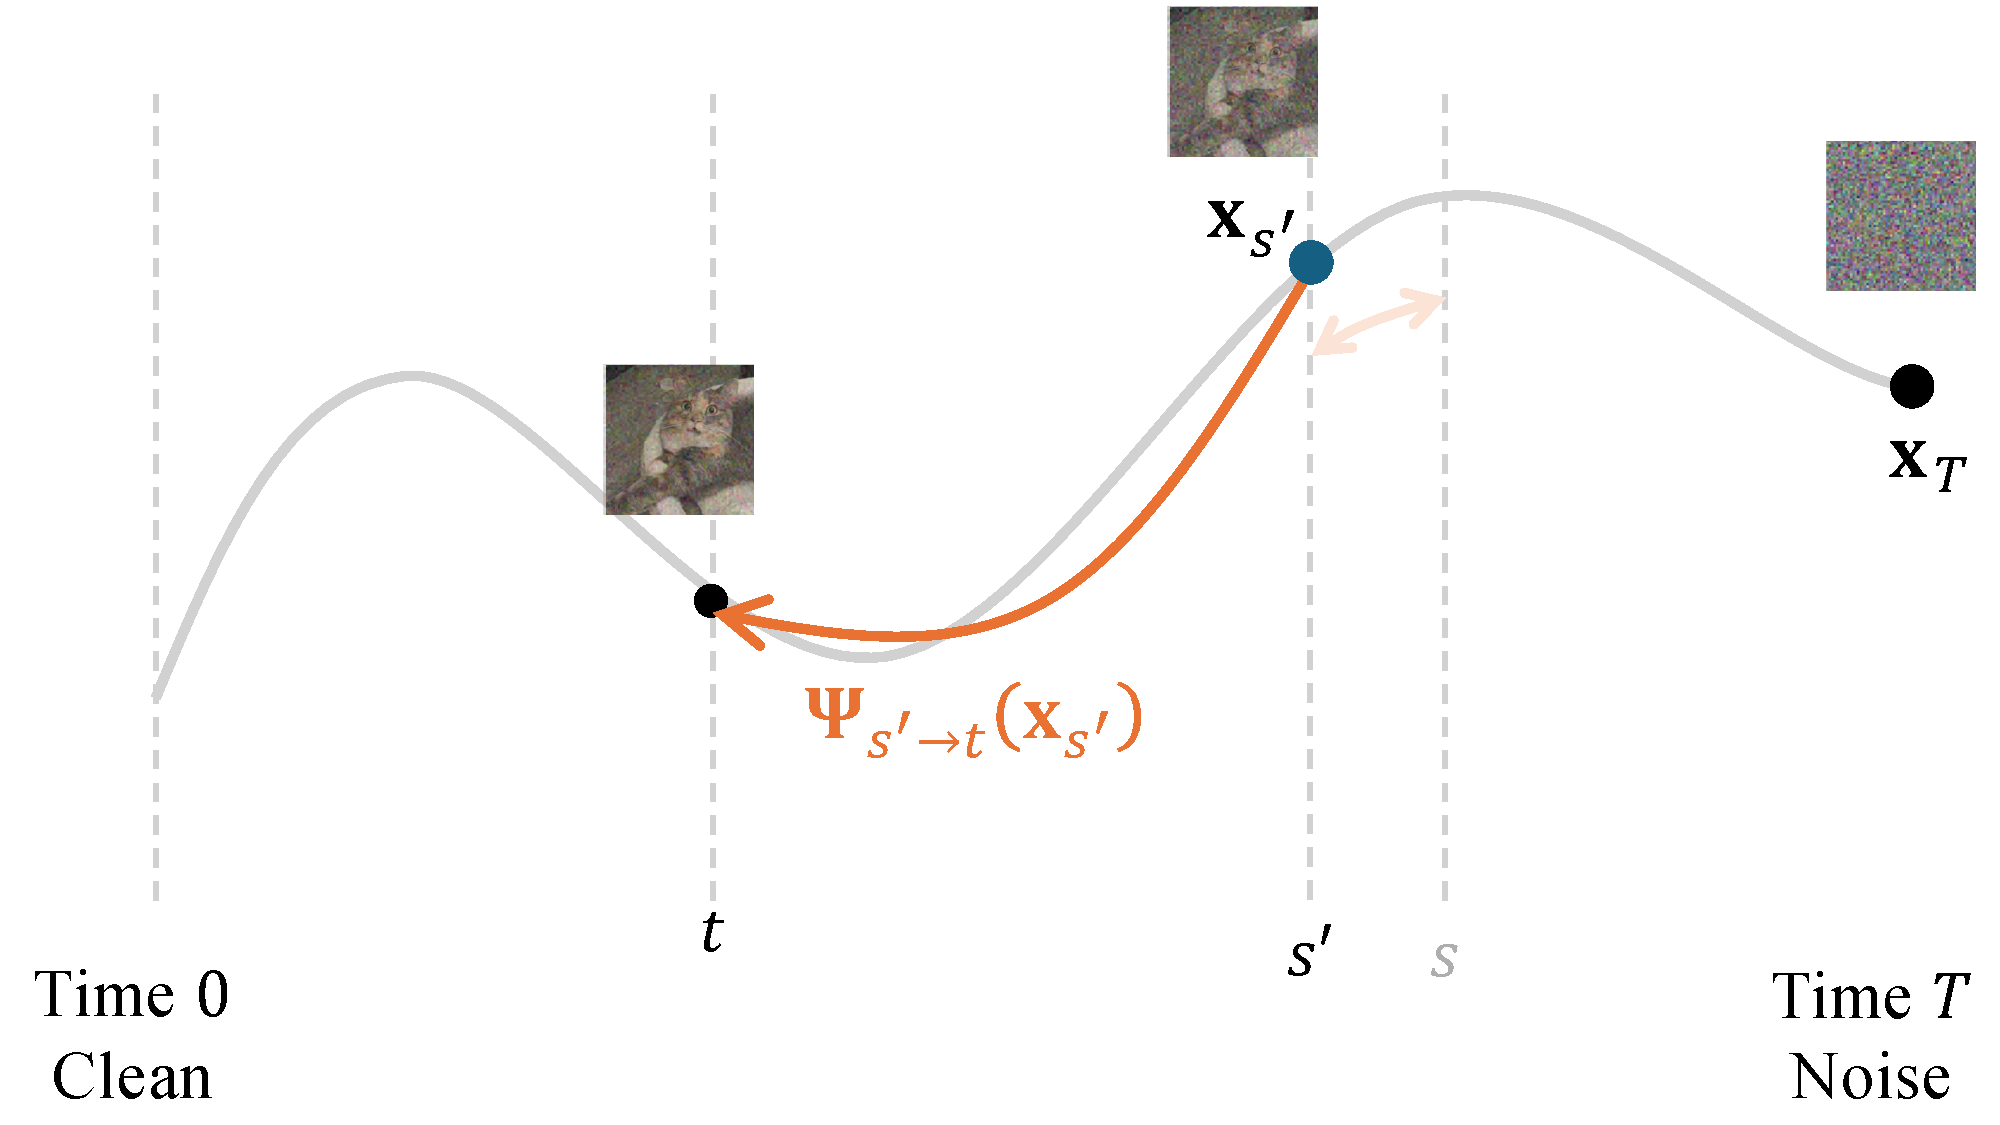
\includegraphics[width=\linewidth]{Images/PartD/eulerian-2.pdf}
        \caption{移动启动时间 $s'$.}
        \label{fig:eulerian-moved}
    \end{subfigure}\caption{\textbfs{E流映射的ulerian一致性。}
    结束时间 $t$ 固定，而开始时间从 $s$ 移至
    $s'$。由于相应的起点位于同一个 PF-ODE 上
轨迹，终点保持不变：
    $\bPsi_{s\to t}(\rvx_s)=\bPsi_{s'\to t}(\rvx_{s'})$。
    无穷小地，这给出
    $\frac{\diff}{\diff s}\bPsi_{s\to t}(\rvx_s)=0$，或同等水平
    $\partial_s\bPsi_{s\to t}(\rvx_s)
    +(\partial_{\rvx}\bPsi_{s\to t})(\rvx_s)\rvv^*(\rvx_s,s)=0$.}
        \figcredit{改编自\citet{dieleman2026flowmaps}.}
    \label{fig:eulerian-consistency}
\end{figure}

\paragraph{三视角的数学等价.}
对于精确的 ODE 流，半群、拉格朗日和欧拉恒等式
都表达了同一个简单的原则：在标准存在下，
唯一性和平滑性假设，ODE 确定唯一性
通过每个状态-时间对的轨迹。也就是说，一旦某个状态
给定的时间是固定的，只有一条路可以走。半群观点
将该路径分成连续的部分，拉格朗日视图遵循其
终点随着结束时间的变化而变化，欧拉观点移动
沿着相同路径的起点，同时保持终点固定。
因此，这三个恒等式是同一 ODE 的等价描述
流~\citep{arnold1988geometrical,chorin1993mathematical}。他们的
通过将半群恒等式视为
有限区间陈述以及拉格朗日和欧拉恒等式
作为它的两个无穷小形式，通过缩小接近结束时间或接近结束时间的短间隔而获得
分别为开始时间。

半群恒等式给出了该原理的有限区间形式：
\[
    \bPsi_{u\to t}\big(\bPsi_{s\to u}(\rvx_s)\big)
    =
    \bPsi_{s\to t}(\rvx_s),
    \qquad
    \bPsi_{s\to s}=\rmI .
\]
通过缩小两个区间之一来获得两个差分视图。

\subparagraph{结束时间限制：拉格朗日恒等式。}
修复起始状态-时间对 $(\rvx_s,s)$ 并缩小最终状态
旅行的一部分。对于$\Delta t>0$，
\[
    \bPsi_{t\to t-\Delta t}
    \big(\bPsi_{s\to t}(\rvx_s)\big)
    =
    \bPsi_{s\to t-\Delta t}(\rvx_s).
\]
让$\rvx_t:=\bPsi_{s\to t}(\rvx_s)$。  Short 的一阶展开式
流给出
\[
    \bPsi_{t\to t-\Delta t}(\rvx_t)
    =
    \rvx_t-\Delta t\,\rvv^*(\rvx_t,t)
    +\mathcal{O}\big((\Delta t)^2\big).
\]
因此，
\[
    \frac{
    \bPsi_{s\to t-\Delta t}(\rvx_s)
    -
    \bPsi_{s\to t}(\rvx_s)}
    {-\Delta t}
    =
    \rvv^*(\rvx_t,t)
    +\mathcal{O}(\Delta t).
\]
采用 $\Delta t\to0$ 得出拉格朗日恒等式
\[
    \partial_t\bPsi_{s\to t}(\rvx_s)
    =
    \rvv^*\big(\bPsi_{s\to t}(\rvx_s),t\big).
\]
因此，当起始状态-时间对 $(\rvx_s,s)$ 固定并且
结束时间改变，结束点随 ODE 速度移动
当时评价的。

\subparagraph{开始时间限制：欧拉恒等式。} 现在固定结束时间 $t$ 并移动开始状态-时间对
沿着相同的轨迹向后移动一个短间隔 $\Delta s>0$：
\[
    \rvx_{s-\Delta s}
    :=
    \bPsi_{s\to s-\Delta s}(\rvx_s)
    =
    \rvx_s-\Delta s\,\rvv^*(\rvx_s,s)
    +\mathcal{O}\big((\Delta s)^2\big).
\]
半群恒等式给出
\[
    \bPsi_{s-\Delta s\to t}(\rvx_{s-\Delta s})
    =
    \bPsi_{s\to t}(\rvx_s).
\]
在起始状态和起始时间下展开左侧可得出
\[
    \bPsi_{s-\Delta s\to t}(\rvx_{s-\Delta s})
    =
    \bPsi_{s\to t}(\rvx_s)
    -
    \Delta s\,
    \big(\partial_{\rvx}\bPsi_{s\to t}\big)(\rvx_s)\rvv^*(\rvx_s,s)
    -
    \Delta s\,
    \partial_s\bPsi_{s\to t}(\rvx_s)
    +
    \mathcal{O}\big((\Delta s)^2\big).
\]
与半群恒等式比较并除以 $-\Delta s$ 得到
\[
    \partial_s\bPsi_{s\to t}(\rvx_s)
    +
    \big(\partial_{\rvx}\bPsi_{s\to t}\big)(\rvx_s)\rvv^*(\rvx_s,s)
    =
    \mathcal{O}(\Delta s).
\]
采用 $\Delta s\to0$ 产生欧拉恒等式
\[
    \partial_s\bPsi_{s\to t}(\rvx_s)
    +
    \big(\partial_{\rvx}\bPsi_{s\to t}\big)(\rvx_s)\rvv^*(\rvx_s,s)
    =
    0.
\]
这里，结束时间$t$是固定的，而起始状态-时间对
沿着相同的轨迹移动。因此终点仍然是
不变。\subparagraph{从任一差异恒等式恢复流映射。}
相反，无论是差分恒等式
与边界条件 $\bPsi_{s\to s}=\rmI$ 一起恢复相同
流映射。  拉格朗日恒等式将终点从
$\bPsi_{s\to s}(\rvx_s)=\rvx_s$。  欧拉恒等式表明
$\bPsi_{\tau\to t}(\rvx_\tau)$沿特性恒定
$\rvx_\tau=\bPsi_{s\to \tau}(\rvx_s)$，因此
\[
    \bPsi_{s\to t}(\rvx_s)
    =
    \bPsi_{t\to t}(\rvx_t)
    =
    \rvx_t.
\]
尽管这些观点在预言机层面是等效的，但它们导致
一旦引入近似值，就会出现不同的实用算法：必须
选择要强制执行的恒等式、在何处放置停止梯度目标、如何
采样时间对，以及如何参数化映射。


\paragraph{关闭.}
本章探讨的中心转变是学习局部速度
领域来学习其 ODE 解映射的有限部分。一个常规的
扩散采样器反复评估局部场并进行数值计算
整合它。相反，流映射模型分摊了此集成的一部分
在训练过程中，可以用一个或几个来遍历很长的区间
网络评价。

这创造了一条快速生成的直接途径，但将困难从
抽样进入学习。该模型必须近似一个更全局的对象，并且
它的成功取决于映射的参数化、
易于处理的目标、时间对的采样和加权以及
优化的稳定性。

从这个角度来看，流映射学习并不是一个新的动态概念，而是一个新的动态概念。
围绕经典学习策略建立的现代学习策略。它保留了
基于轨迹的扩散模型基础，同时扩大设计
高效生成的空间。目标不再只是整合
生成 ODE 在推理时更有效，但学习有用
直接对其解映射进行有限时间转换。





























\clearpage
\newpage